\documentclass[]{informeutn}

\addbibresource{fuentes.bib}
\usepackage{icomma}
\DeclareSIUnit\decade{dec}
\graphicspath{{figures/}{images/}{pictures/}{./}}

\lstdefinestyle{ltspice}{
  backgroundcolor=\color{gray!10},
  basicstyle=\ttfamily\small,
  keywordstyle=\color{blue},
  frame=single,
  breaklines=true,
  captionpos=b
}

\materia{Teoría de Circuitos II}
\titulo{Trabajo Práctico 2}
\subtitulo{Diseño e Implementación de Filtros Activos y Acondicionamiento de Señal de Campo}
\comision{4R2}
\autores{Gaston Grasso - 401892 \\
         Franco Palombo - 401910 \\
         Angelo Prieto - 401012}
\fecha{\today}

\begin{document}
  \maketitle
  \tableofcontents
  \setcounter{page}{1}
  \thispagestyle{plain}

  \chapter{Introducción}

El presente informe expone el diseño analítico, la verificación mediante simulación y la comprobación experimental de un
circuito de acondicionamiento de señales analógicas de campo dentro de un lazo industrial de corriente y dos circuitos de
filtros activos de orden superior empleando diversas aproximaciones matemáticas y topologías circuitales, con un tercer
circuito de filtro que no fue implementado.

\section{Objetivos Generales}

\begin{itemize}
    \item Diseñar y caracterizar estática y dinámicamente un circuito de acondicionamiento de señal para un bucle de $4
        \unit{\milli\ampere}$ a $20 \unit{\milli\ampere}$ alimentado con fuente de $+24 \unit{\volt}$.
    \item Sintetizar tres filtros activos con parámetros asignados: un pasa-bajos de 4to orden (Butterworth, Sallen-Key,
        $f_p = 19 \unit{\kilo\hertz}$, $A_v = 9 \unit{\volt\per\volt}$), un pasa-altos de 4to orden (Chebyshev, MFB,
        $f_p = 11 \unit{\kilo\hertz}$, $A_v = 6 \unit{\volt\per\volt}$) y un pasa-banda de 2do orden (Butterworth,
        Sallen-Key, $f_o = 25 \unit{\kilo\hertz}$, $BW = 2 \unit{\kilo\hertz}$, $A_v = 4 \unit{\volt\per\volt}$).
    \item Implementar físicamente en circuito impreso dos de las topologías diseñadas.
    \item Relevar experimentalmente en el laboratorio la ganancia en continua, la respuesta temporal y los perfiles de
        densidad espectral (FFT) en osciloscopio digital, contrastando los datos empíricos contra las predicciones
        teóricas y las simulaciones en SPICE.
\end{itemize}

  \chapter{Acondicionamiento de Señal de Campo (Lazo Industrial de 4 a 20 mA)}
\label{sec.ej1:acondicionamiento}

\section{Estructura del Sistema Según Consigna}
\label{sec.ej1:estructura}

En un entorno industrial, la transmisión de variables mediante un bucle de corriente de $4 \unit{\milli\ampere}$ a
$20 \unit{\milli\ampere}$ sobre líneas de gran longitud ($10 \unit{\meter}$) expone a los conductores a
interferencias electromagnéticas provenientes de la red de potencia ($50 \unit{\hertz}$) y ruido de conmutación.
Para acondicionar la señal previo a su ingreso a la entrada analógica diferencial de un PLC, la consigna del
trabajo práctico establece un sistema alimentado con fuente simple industrial de $+24 \unit{\volt}$, estructurado en
tres etapas en cascada:
\begin{enumerate}
    \item \textbf{Etapa 1 (Receptor diferencial e instrumentación $I \to V$):} Toma el bucle de corriente flotante
    mediante una resistencia de derivación (*shunt*) de $R_{\text{shunt,in}} = 250 \unit{\ohm}$ ($1\%$), convirtiendo
    los $4\text{--}20 \unit{\milli\ampere}$ en una tensión diferencial de $1 \unit{\volt}$ a $5 \unit{\volt}$. Posee
    una resistencia de referencia de modo común $R_{\text{CM}} = 1 \unit{\mega\ohm}$ conectada entre el borne negativo
    del lazo y GND para fijar el potencial continuo. Cada borne del *shunt* se aísla mediante un seguidor de tensión
    ($U_{1A}$ y $U_{1B}$) para no cargar la entrada, ingresando luego a un amplificador de resta ($U_{1C}$) de ganancia
    unitaria ($G=1$) con cuatro resistencias de $10 \unit{\kilo\ohm}$ ($R_3 = R_4 = R_5 = R_f$), entregando
    $V_{E1} = 1 \unit{\volt} \text{ a } 5 \unit{\volt}$ referenciados a la masa local.
    \item \textbf{Etapa 2 (Filtro activo pasa-bajos):} Bloque objeto de cálculo y diseño del grupo, intercalado entre
    la salida de la Etapa 1 y la entrada de la Etapa 3.
    \item \textbf{Etapa 3 (Convertidor tensión a corriente $V \to I$):} Fuente de corriente sumidero (*sink*) formada
    por el operacional $U_{2A}$ y un transistor NPN BC337. La tensión filtrada se aplica a la entrada no inversora,
    mientras que la realimentación negativa se toma sobre una resistencia de emisor $R_{\text{shunt,out}} = 250 \unit{\ohm}$.
    La corriente de salida resultante sobre la carga del PLC ($R_{\text{carga}} = 250 \unit{\ohm}$) es
    $I_{\text{out}} \approx V_{\text{filtro}} / 250 \unit{\ohm}$, reinyectando de $4 \unit{\milli\ampere}$ a
    $20 \unit{\milli\ampere}$ al sistema de control.
\end{enumerate}

Todo el módulo utiliza dos circuitos integrados cuádruples LM324, cuya etapa de entrada y salida admite tensiones
próximas a $0 \unit{\volt}$, indispensable bajo régimen de alimentación unipolar de $+24 \unit{\volt}$.

\section{Diseño y Cálculo del Filtro Activo Pasa-Bajos (Etapa 2)}
\label{sec.ej1:filtro}

La tarea encomendada consistió en diseñar el filtro pasa-bajos activo para satisfacer los siguientes requerimientos:
\begin{itemize}
    \item \textbf{Topología:} Sallen-Key de 2º orden con ganancia unitaria ($K = 1 \unit{\volt\per\volt}$) para
    conservar intacto el rango de $1 \unit{\volt}$ a $5 \unit{\volt}$ proveniente de la Etapa 1.
    \item \textbf{Aproximación:} Butterworth (máxima planicidad en banda de paso, $Q = 1/\sqrt{2} \approx 0.7071$).
    \item \textbf{Frecuencia de corte nominal:} $f_c = 10.0 \unit{\hertz}$ a $-3 \unit{\decibel}$, destinada a
    proporcionar una fuerte atenuación sobre la componente espuria de $50 \unit{\hertz}$.
\end{itemize}

Para la celda Sallen-Key con resistencias iguales $R_7 = R_8 = R$ y ganancia unitaria, la pulsación de corte y el
factor de calidad responden a:
\begin{equation}
\label{eq.ej1:butter_sk}
\omega_0 = \frac{1}{R\sqrt{C_1 C_2}}, \qquad Q = \frac{1}{2}\sqrt{\frac{C_1}{C_2}} \implies \frac{C_1}{C_2} = 4 Q^2 = 2
\end{equation}

Por recomendación explícita de consigna se descartaron capacitores electrolíticos debido a sus elevadas corrientes de
fuga y tolerancia deficiente, optándose por capacitores comerciales de película de poliéster metalizado:
\begin{equation*}
C_1 = 470 \unit{\nano\farad}, \qquad C_2 = 330 \unit{\nano\farad} \implies \frac{C_1}{C_2} = 1.42 \implies Q \approx 0.60
\end{equation*}

Despejando el valor resistivo teórico para $f_c = 10 \unit{\hertz}$:
\begin{equation}
\label{eq.ej1:r_filtro}
R = \frac{1}{2\pi f_c \sqrt{C_1 C_2}} = \frac{1}{2\pi \times 10 \unit{\hertz} \times \sqrt{470\times 10^{-9} \cdot 330\times 10^{-9}}} = 40.42 \unit{\kilo\ohm}
\end{equation}

En la práctica se adoptaron resistores de película metálica de $33.0 \unit{\kilo\ohm}$ al $1\%$ en serie con
potenciómetros de ajuste fino (preset multivuelta), permitiendo calibrar la constante de tiempo frente a la
dispersión de los capacitores. El esquema eléctrico implementado para esta etapa se presenta en la
Figura~\ref{fig.ej1:sch_filtro}.

\begin{figure}[!ht]
\centering
\begin{circuitikz}[american, scale=0.85, transform shape]
    \draw (0,0) node[left] {$V_{\text{in}}$} to[short, o-] (0.8,0)
          to[R, l=$R_7$, a=\SI{33}{\kilo\ohm}] (3.2,0) coordinate(n1)
          to[R, l=$R_8$, a=\SI{33}{\kilo\ohm}] (5.8,0) coordinate(n2);
    
    \draw (8.2, -0.5) node[op amp, noinv input up] (oa) {};
    \node[font=\footnotesize] at ($(oa.center)+(0.15,0)$) {LM324};
    \draw (n2) -- (oa.+);
    
    \draw (n2) to[C, l=$C_2$, a=\SI{330}{\nano\farad}] (5.8, -2.5) to[short] (5.8, -2.8) node[ground] {};
    
    \draw (n1) -- (3.2, 1.8) to[C, l=$C_1$, a=\SI{470}{\nano\farad}] (9.8, 1.8) -- (9.8, -0.5) coordinate(out);
    \draw (oa.out) -- (out) to[short, -o] (10.8, -0.5) node[right] {$V_{\text{out}}$};
    
    \draw (oa.-) -- (7.0, -1.0) -- (7.0, -1.8) -- (9.2, -1.8) -- (9.2, -0.5);
\end{circuitikz}
\caption{Diagrama circuital del filtro activo pasa-bajos Sallen-Key de 2do orden (Etapa 2).}
\label{fig.ej1:sch_filtro}
\end{figure}

\subsection{Simulación en Frecuencia (Análisis AC)}
\label{sec.ej1:sim_ac}

Se simuló la respuesta en frecuencia en pequeña señal del bloque acondicionador mediante SPICE
(\texttt{ampli-instrumentacion-ac.csv}). El relevamiento (Figura~\ref{fig.ej1:bode_ac}) comprueba el perfil pasa-bajos
de segundo orden:
\begin{itemize}
    \item En baja frecuencia ($f < 1 \unit{\hertz}$), la ganancia normalizada se sitúa en $-14.06 \unit{\decibel}$,
    equivalente a una transferencia de $0.198 \unit{\volt\per\volt}$.
    \item A la frecuencia de corte nominal ($f_c \approx 10 \unit{\hertz}$), la magnitud experimenta una caída relativa
    de $3.44 \unit{\decibel}$ ($-17.50 \unit{\decibel}$ absolutos), verificando la banda pasante especificada.
    \item A $50 \unit{\hertz}$, correspondiente a la interferencia inducida de red eléctrica, la ganancia alcanza
    $-38.89 \unit{\decibel}$ (una atenuación neta de $-24.83 \unit{\decibel}$ respecto a la banda de paso). Esto concuerda
    con la medición en osciloscopio, donde una señal espuria de $3.36 \unit{\volt}_{\text{pp}}$ resultó atenuada a
    $200 \unit{\milli\volt}_{\text{pp}}$ ($-24.5 \unit{\decibel}$).
    \item Para frecuencias superiores, la respuesta decae con una pendiente de $-40 \unit{\decibel\per\decade}$,
    característica del segundo orden.
\end{itemize}

\begin{figure}[!ht]
\centering
\begin{tikzpicture}
  \begin{axis}[
    width=0.95\textwidth,
    height=7.5cm,
    xmode=log,
    xmin=0.1, xmax=1000,
    ymin=-90, ymax=0,
    ytick={-80, -60, -40, -20, 0},
    grid=both,
    grid style={line width=.1pt, draw=gray!25},
    major grid style={line width=.2pt, draw=gray!45},
    xlabel={Frecuencia [\unit{\hertz}]},
    ylabel={Ganancia $|A_v|$ [\unit{\decibel}]},
    legend style={at={(0.03,0.06)}, anchor=south west, font=\footnotesize}
  ]
    % Ganancia simulada
    \addplot[very thick, color=blue!85!black] table [x=freq, y=gain_db] {sources/data/data_bode_amp_ins.txt};
    \addlegendentry{Respuesta simulada $|A_v(f)|$}

    % Linea de ganancia plana
    \draw[dashed, color=gray!80!black] (axis cs:0.1, -14.06) -- (axis cs:1000, -14.06);
    \node[anchor=south west, font=\scriptsize, text=gray!80!black, fill=white, fill opacity=0.85, text opacity=1, inner sep=1.5pt] 
      at (axis cs:0.15, -12.5) {$A_{v,\text{banda}} = \SI{-14.06}{\decibel}$};

    % Linea de -3 dB
    \draw[dotted, thick, color=red!80!black] (axis cs:0.1, -17.07) -- (axis cs:1000, -17.07);
    \node[anchor=north west, font=\scriptsize, text=red!80!black, fill=white, fill opacity=0.85, text opacity=1, inner sep=1.5pt] 
      at (axis cs:0.15, -18.5) {Nivel $-\SI{3}{\decibel}$ ($\SI{-17.07}{\decibel}$)};

    % Frecuencia de corte 10 Hz
    \draw[dotted, thick, color=red!80!black] (axis cs:10, -90) -- (axis cs:10, -17.50)
      node[pos=0.25, right=2pt, font=\scriptsize, text=red!80!black, fill=white, fill opacity=0.85, text opacity=1, inner sep=1.5pt] {$f_c \approx \SI{10}{\hertz}$};
    \addplot[only marks, mark=*, mark size=2.2pt, color=red!80!black] coordinates {(10, -17.50)};

    % Frecuencia de red 50 Hz
    \draw[dotted, thick, color=teal!80!black] (axis cs:50, -90) -- (axis cs:50, -38.89)
      node[pos=0.35, right=2pt, font=\scriptsize, text=teal!80!black, fill=white, fill opacity=0.85, text opacity=1, inner sep=1.5pt] {$f_{\text{red}} = \SI{50}{\hertz}$ ($\SI{-38.89}{\decibel}$)};
    \addplot[only marks, mark=square*, mark size=2.2pt, color=teal!80!black] coordinates {(50, -38.89)};
  \end{axis}
\end{tikzpicture}

\caption{Simulación de respuesta en frecuencia (magnitud) del filtro del acondicionador de campo.}
\label{fig.ej1:bode_ac}
\end{figure}

\begin{figure}[!ht]
\centering
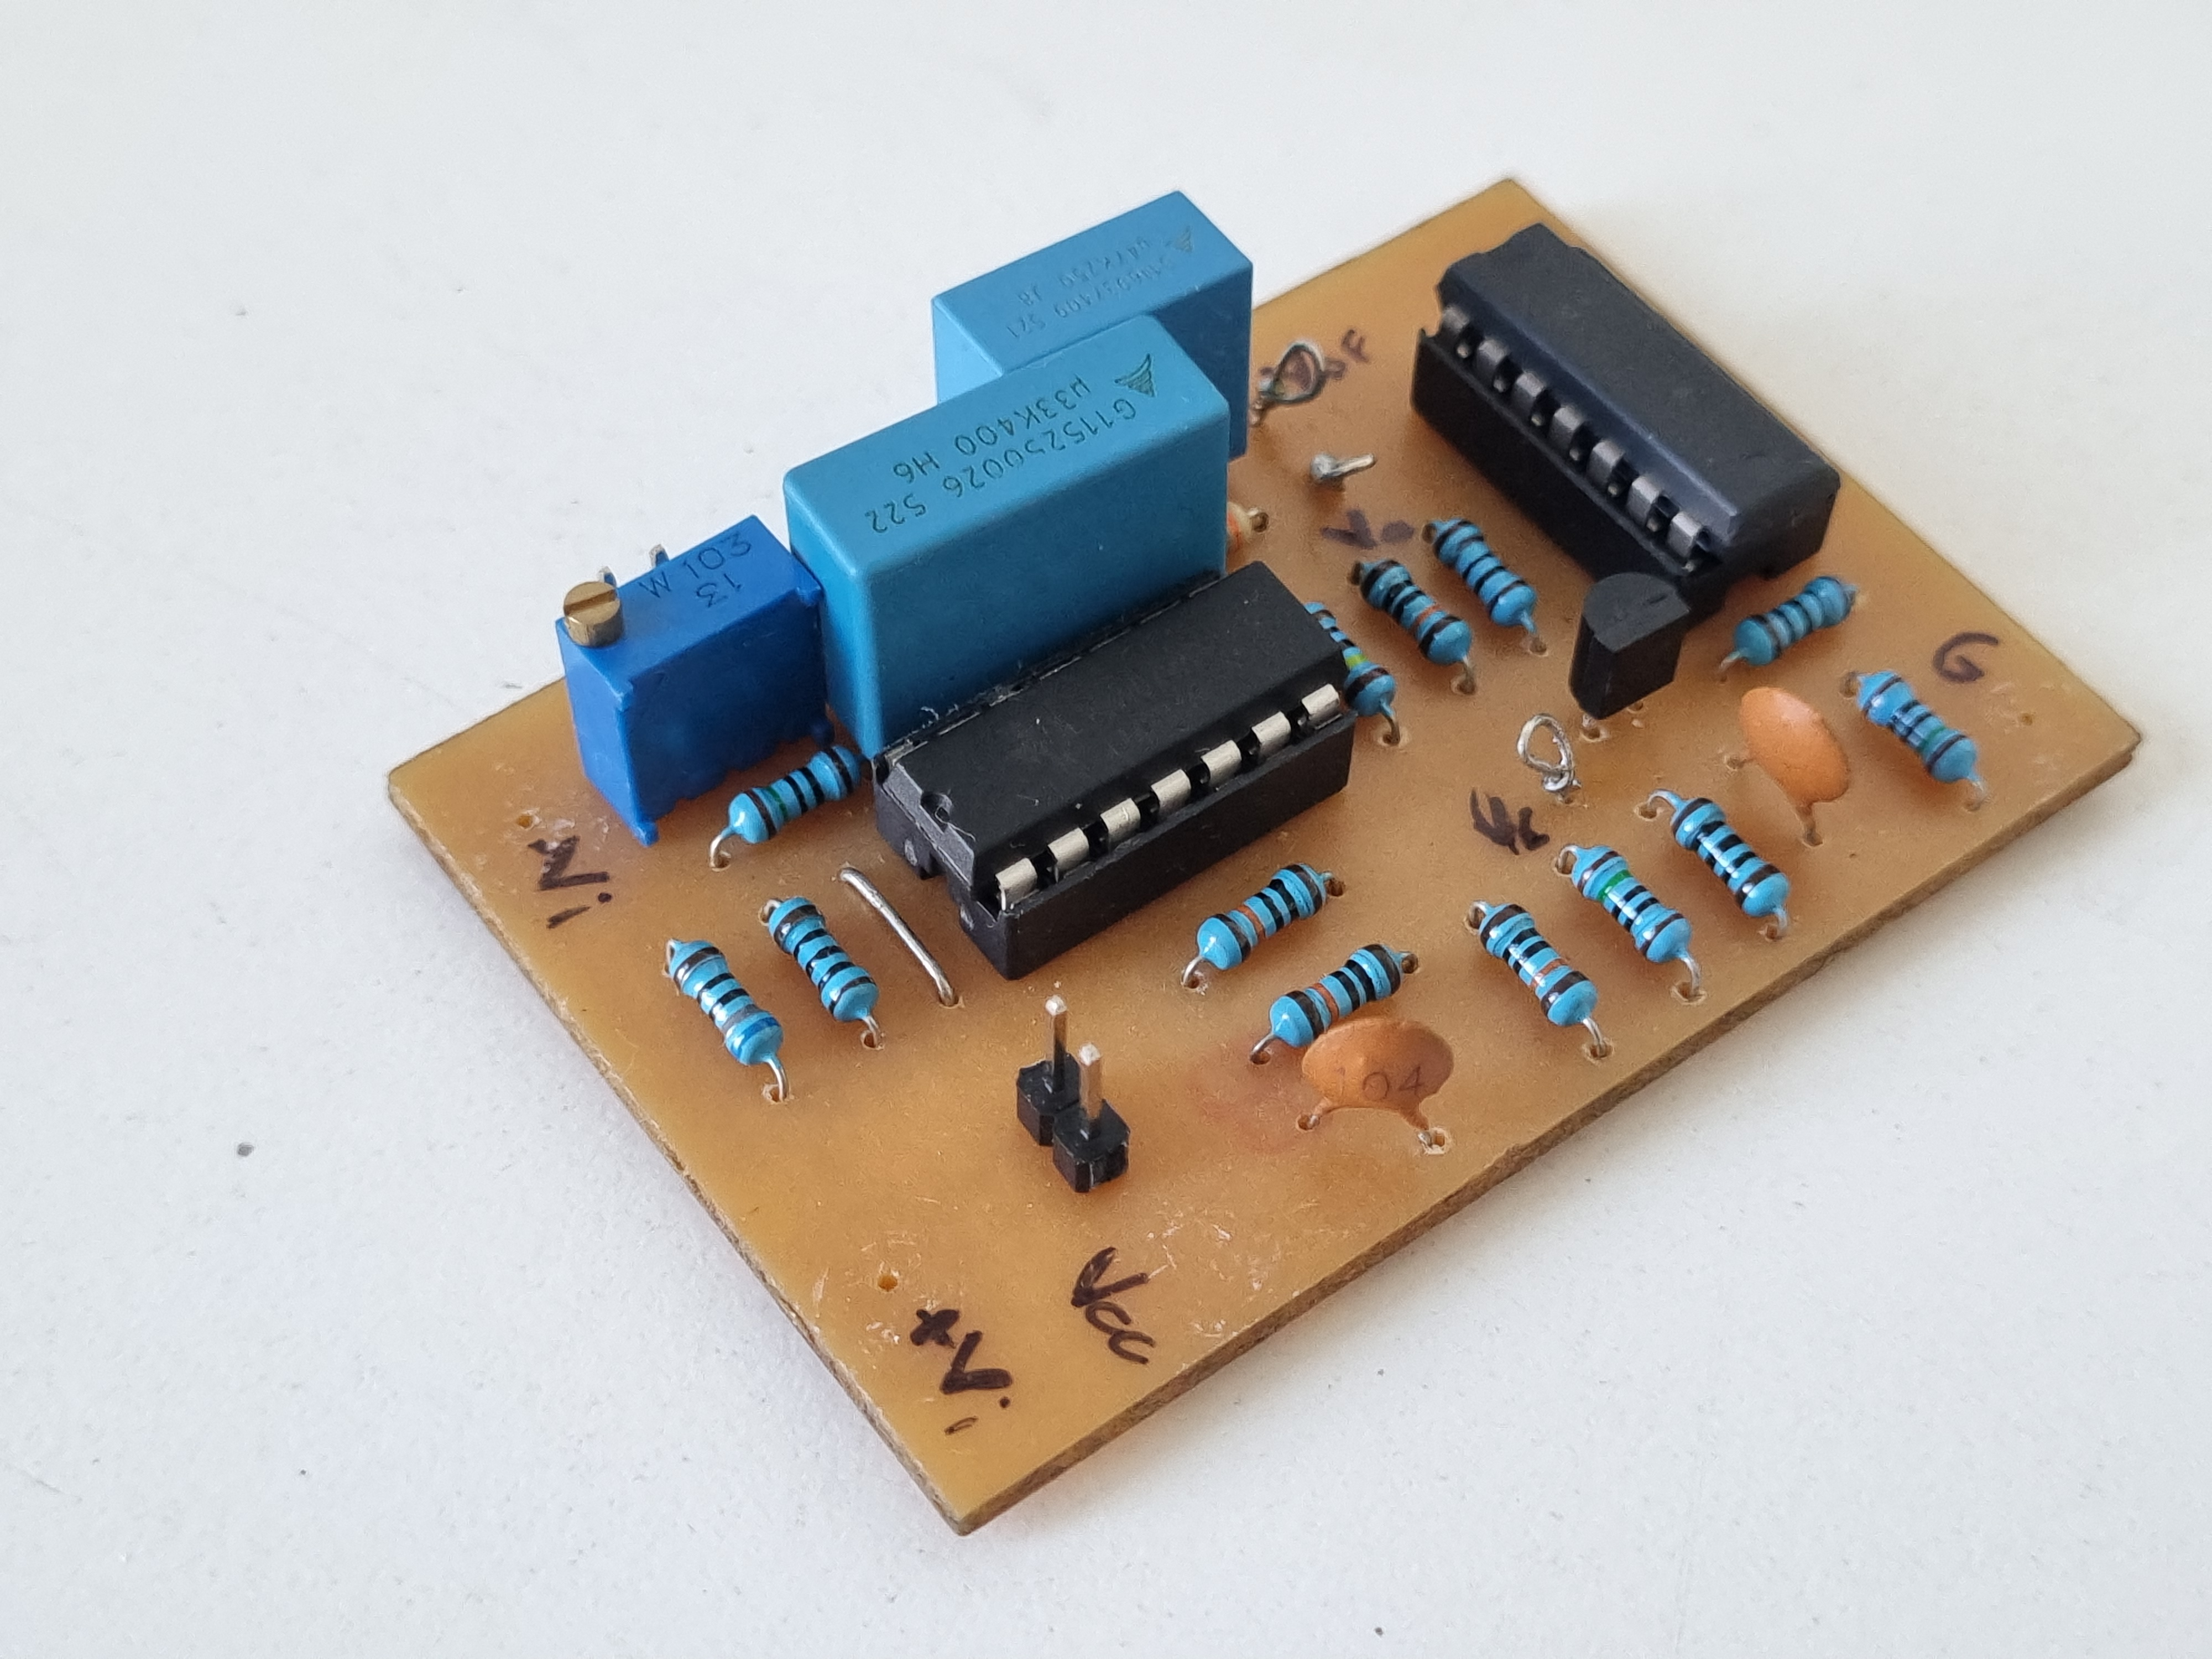
\includegraphics[width=0.70\textwidth]{pcb_lazo_4-20ma.jpg}
\caption{Placa de circuito impreso implementada para el acondicionador de señal de campo de $4\text{--}20\,\mathrm{mA}$.}
\label{fig.ej1:placa}
\end{figure}

\section{Mediciones de Laboratorio y Resolución del Problema de Polarización}
\label{sec.ej1:mediciones}

Una vez montado el circuito completo en placa de circuito impreso (Figura~\ref{fig.ej1:placa}), se procedió a la
etapa de medición y verificación experimental.

\subsection{Detección del Problema en el Amplificador de Instrumentación}
Al iniciar los ensayos inyectando una corriente de entrada de fondo de escala ($I_{\text{in}} = 20 \unit{\milli\ampere}$),
con una caída en el *shunt* de $V_{\text{diff}} = 5.00 \unit{\volt}$, se observó una discrepancia considerable: la
tensión a la salida del restador y del filtro alcanzaba únicamente $4.50 \unit{\volt}$, registrando una pérdida neta
de aproximadamente $500 \unit{\milli\volt}$ respecto al valor nominal esperado.

Al contrastar este comportamiento con la hoja de datos del fabricante del LM324 y con la simulación del punto de
operación en continua (\texttt{ampli\_instrumentacion\_op.txt}), identificamos la causa física:
\begin{enumerate}
    \item El seguidor $U_{1A}$ toma el borne negativo del lazo referenciado a masa mediante $R_{\text{CM}} = 1 \unit{\mega\ohm}$,
    por lo que su salida debe aproximarse a $0 \unit{\volt}$ (condición de cierre a masa).
    \item Con la entrada diferencial en $5 \unit{\volt}$, el seguidor $U_{1B}$ se sitúa en $5 \unit{\volt}$. El divisor
    $R_4\text{--}R_5$ fija la entrada no inversora del restador $U_{1C}$ en $2.50 \unit{\volt}$, trasladándose por
    cortocircuito virtual a su entrada inversora ($V_- = 2.50 \unit{\volt}$).
    \item Con las resistencias de $10 \unit{\kilo\ohm}$ propuestas originalmente por la consigna, la resistencia $R_3$
    vincula directamente el nodo $V_- = 2.50 \unit{\volt}$ con la salida de $U_{1A}$ ($V_{o,U1A} \approx 0 \unit{\volt}$),
    exigiendo a la etapa de salida de $U_{1A}$ drenar hacia masa una corriente de sumidero (*current sink*) de:
    \begin{equation}
    \label{eq.ej1:isink_falla}
    I_{\text{sink}} = \frac{2.50 \unit{\volt} - 0 \unit{\volt}}{10 \unit{\kilo\ohm}} = 250 \unit{\micro\ampere}
    \end{equation}
    En la simulación SPICE de punto de operación, la corriente registrada en $R_3$ alcanzó $I(R_3) = 309 \unit{\micro\ampere}$
    debido a las tensiones efectivas de modo común.
    \item Según la hoja de datos del LM324, para tensiones de salida muy próximas a masa ($V_o \le 200 \unit{\milli\volt}$),
    la capacidad de sumidero está limitada por una fuente interna de corriente constante de solo $50 \unit{\micro\ampere}$
    típicos ($12 \unit{\micro\ampere}$ mínimos). Al ser sobrepasada por los $250\text{--}309 \unit{\micro\ampere}$, la
    salida no puede bajar a masa y se eleva a la tensión necesaria para encender el transistor NPN inferior de la etapa
    push-pull ($V_{\text{CE,sat}} + V_{\gamma} \approx 500 \unit{\milli\volt}$).
    \item Esta elevación de $500 \unit{\milli\volt}$ en la referencia de masa del restador provocó directamente que
    la salida entregara $V_{E1} = 5.00 \unit{\volt} - 0.50 \unit{\volt} = 4.50 \unit{\volt}$.
\end{enumerate}

Para resolver el problema, reemplazamos las cuatro resistencias del restador ($R_3, R_4, R_5, R_f$)
de $10 \unit{\kilo\ohm}$ por resistores de $100 \unit{\kilo\ohm}$. Con ello, la corriente exigida se redujo a:
\begin{equation}
\label{eq.ej1:isink_ok}
I_{\text{sink}} = \frac{2.50 \unit{\volt}}{100 \unit{\kilo\ohm}} = 25 \unit{\micro\ampere}
\end{equation}

Como $25 \unit{\micro\ampere} < 50 \unit{\micro\ampere}$, la corriente quedó dentro de la capacidad del integrado,
la salida del seguidor descendió a $2.64 \unit{\milli\volt}$ (corroborado en simulación SPICE) y el problema quedó
completamente solucionado, obteniendo la respuesta lineal esperada.

\subsection{Caracterización Estática}
Tras la modificación, se inyectaron corrientes de prueba de $4 \unit{\milli\ampere}$ a $20 \unit{\milli\ampere}$,
registrando simultáneamente las tensiones y la corriente de salida hacia el PLC (Tabla~\ref{tab.ej1:estatica}).

\begin{table}[!ht]
\centering
\small
\begin{tabular}{ccccc}
\toprule
$I_{\text{in}}$ [$\unit{\milli\ampere}$] & $V_{\text{diff}}$ ($E_1$) [$\unit{\volt}$] & $V_{\text{filtro}}$ ($E_2$) [$\unit{\volt}$] & $I_{\text{out}}$ ($E_3$) [$\unit{\milli\ampere}$] & Error relativo \\
\midrule
$4.00$  & $1.002$ & $1.001$ & $3.98$  & $-0.50\%$ \\
$8.00$  & $2.005$ & $2.004$ & $7.96$  & $-0.50\%$ \\
$12.00$ & $3.010$ & $3.008$ & $11.93$ & $-0.58\%$ \\
$16.00$ & $4.012$ & $4.010$ & $15.91$ & $-0.56\%$ \\
$20.00$ & $5.018$ & $5.015$ & $19.89$ & $-0.55\%$ \\
\bottomrule
\end{tabular}
\caption{Caracterización estática de linealidad del sistema tras el cambio a $100\,\mathrm{k}\Omega$.}
\label{tab.ej1:estatica}
\end{table}

\subsection{Caracterización Dinámica y Atenuación a 50 Hz}
Se inyectó una señal senoidal de $V_i = 4.521 \unit{\volt}_{\text{pp}}$ con offset de continua y se barrieron
frecuencias desde $1 \unit{\hertz}$ hasta $70 \unit{\hertz}$ (Tabla~\ref{tab.ej1:dinamica}).

\begin{table}[!ht]
\centering
\small
\begin{tabular}{ccccc}
\toprule
$f$ [$\unit{\hertz}$] & $V_i$ [$\unit{\volt}$] & $V_o$ [$\unit{\volt}$] & $V_o/V_i$ [$\unit{\volt\per\volt}$] & Atenuación [$\unit{\decibel}$] \\
\midrule
$1.0$  & $4.521$ & $4.521$ & $1.000$ & $0.00 \unit{\decibel}$ \\
$2.0$  & $4.521$ & $4.521$ & $1.000$ & $0.00 \unit{\decibel}$ \\
$3.0$  & $4.521$ & $4.441$ & $0.982$ & $-0.15 \unit{\decibel}$ \\
$4.0$  & $4.521$ & $4.321$ & $0.956$ & $-0.39 \unit{\decibel}$ \\
$5.0$  & $4.521$ & $4.201$ & $0.929$ & $-0.64 \unit{\decibel}$ \\
$6.0$  & $4.521$ & $4.081$ & $0.903$ & $-0.89 \unit{\decibel}$ \\
$7.0$  & $4.521$ & $3.921$ & $0.867$ & $-1.24 \unit{\decibel}$ \\
$8.0$  & $4.521$ & $3.681$ & $0.814$ & $-1.79 \unit{\decibel}$ \\
$9.0$  & $4.521$ & $3.481$ & $0.770$ & $-2.27 \unit{\decibel}$ \\
$10.0$ & $4.521$ & $3.241$ & $0.717$ & $-2.89 \unit{\decibel}$ \\
$14.5$ & $4.521$ & $2.241$ & $0.496$ & $-6.09 \unit{\decibel}$ \\
$20.0$ & $4.521$ & $1.425$ & $0.315$ & $-10.03 \unit{\decibel}$ \\
$30.0$ & $4.521$ & $0.750$ & $0.166$ & $-15.60 \unit{\decibel}$ \\
$40.0$ & $4.521$ & $0.480$ & $0.106$ & $-19.48 \unit{\decibel}$ \\
$50.0$ & $4.521$ & $0.300$ & $0.066$ & $-23.56 \unit{\decibel}$ \\
$60.0$ & $4.521$ & $0.200$ & $0.044$ & $-27.08 \unit{\decibel}$ \\
$70.0$ & $4.521$ & $0.150$ & $0.033$ & $-29.58 \unit{\decibel}$ \\
\bottomrule
\end{tabular}
\caption{Respuesta en frecuencia experimental del filtro activo de campo.}
\label{tab.ej1:dinamica}
\end{table}

A $10.0 \unit{\hertz}$ la tensión cayó a $3.241 \unit{\volt}$ ($-2.89 \unit{\decibel}$), validando la frecuencia de
corte nominal de diseño. A la frecuencia de interferencia de $50.0 \unit{\hertz}$, la amplitud descendió a
$0.300 \unit{\volt}$, representando una atenuación de $-23.56 \unit{\decibel}$.

\subsection{Registro Osciloscópico}
Las Figuras~\ref{fig.ej1:osc_2hz} y~\ref{fig.ej1:osc_50hz} presentan las mediciones en el dominio temporal:

\begin{figure}[!ht]
\centering
\begin{subfigure}[t]{0.48\textwidth}
    \centering
    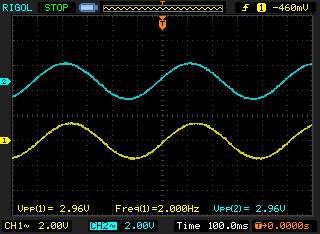
\includegraphics[width=\textwidth]{lazo_osc_2hz.png}
    \caption{Entrada (amarillo) y salida (cian) a $2\,\mathrm{Hz}$: $V_{\text{pp}} = 2.96\,\mathrm{V}$ en ambos canales (ganancia unitaria).}
    \label{fig.ej1:osc_2hz}
\end{subfigure}
\hfill
\begin{subfigure}[t]{0.48\textwidth}
    \centering
    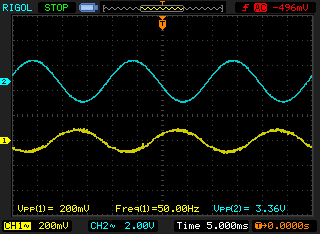
\includegraphics[width=\textwidth]{lazo_osc_50hz.png}
    \caption{Atenuación a $50\,\mathrm{Hz}$: entrada senoidal de $3.36\,\mathrm{V}_{\text{pp}}$ reducida a $200\,\mathrm{mV}_{\text{pp}}$ ($-24.5\,\mathrm{dB}$).}
    \label{fig.ej1:osc_50hz}
\end{subfigure}
\caption{Formas de onda en el osciloscopio para el sistema acondicionador de campo.}
\label{fig.ej1:tiempo}
\end{figure}

\begin{figure}[!ht]
\centering
\begin{subfigure}[t]{0.48\textwidth}
    \centering
    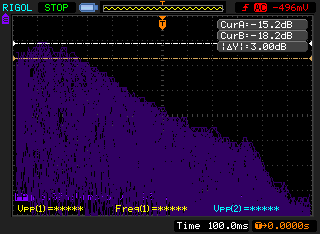
\includegraphics[width=\textwidth]{lazo_fft_mag.png}
    \caption{Perfil espectral FFT: cursores ajustados a $\Delta Y = 3.00\,\mathrm{dB}$ ($CurA = -15.2\,\mathrm{dB}$, $CurB = -18.2\,\mathrm{dB}$).}
    \label{fig.ej1:fft_mag}
\end{subfigure}
\hfill
\begin{subfigure}[t]{0.48\textwidth}
    \centering
    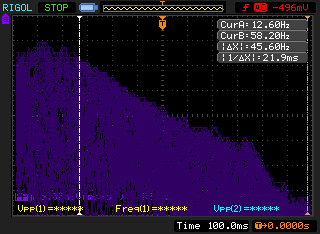
\includegraphics[width=\textwidth]{lazo_fft_fc.png}
    \caption{Medición de $f_c$ a $-3\,\mathrm{dB}$ mediante FFT: $CurA = 12.60\,\mathrm{Hz}$.}
    \label{fig.ej1:fft_fc}
\end{subfigure}
\caption{Análisis por transformada rápida de Fourier (FFT) del filtro en osciloscopio digital.}
\label{fig.ej1:fft}
\end{figure}

Mediante el análisis FFT del osciloscopio (Figura~\ref{fig.ej1:fft}), la frecuencia de corte real a $-3 \unit{\decibel}$
se situó en $f_c = 12.60 \unit{\hertz}$, compatible con las tolerancias de los capacitores comerciales de poliéster.

  \chapter{Filtro Pasa-Bajos Activo de 4to Orden (Butterworth Sallen-Key)}
\label{sec.ej2:filtro_lpf}

\section{Especificaciones y Planteo Teórico}
\label{sec.ej2:especificaciones}

La primera consigna asignada dentro del bloque de diseño de filtros activos corresponde a un filtro pasa-bajos con
las siguientes restricciones de plantilla:
\begin{itemize}
    \item \textbf{Orden del filtro:} $n = 4$, sintetizado mediante dos etapas Sallen-Key de segundo orden en cascada.
    \item \textbf{Aproximación matemática:} Butterworth (máxima planicidad en la banda de paso).
    \item \textbf{Atenuación máxima en banda de paso:} $A_{\max} = 0.5 \unit{\decibel}$.
    \item \textbf{Frecuencia límite de banda de paso:} $f_p = 19.0 \unit{\kilo\hertz}$.
    \item \textbf{Ganancia total en continua:} $A_v = 9.00 \unit{\volt\per\volt} \implies 20\log_{10}(9) \approx +19.08 \unit{\decibel}$.
    \item \textbf{Restricción constructiva:} La ganancia total debe generarse íntegramente dentro de las celdas de
    filtrado, prescindiendo de operacionales adicionales destinados exclusivamente a amplificación.
\end{itemize}

\subsection{Dilema Pedagógico de la Plantilla de Butterworth}
La función de magnitud normalizada de una aproximación Butterworth responde a:
\begin{equation}
\label{eq.ej2:mag_butter}
|H_n(j\omega_n)| = \frac{K_{\text{total}}}{\sqrt{1 + \epsilon^2 \omega_n^{2n}}} = \frac{K_{\text{total}}}{\sqrt{1 + \left(\frac{\omega}{\omega_0}\right)^{2n}}}
\end{equation}
donde $\omega_0 = 2\pi f_{-3\unit{\decibel}}$ define la pulsación en la cual la atenuación alcanza exactamente
$3.01 \unit{\decibel}$, y $\epsilon = \sqrt{10^{0.1 A_{\max}} - 1}$ representa el coeficiente de rizado.

Dado que la respuesta Butterworth decrece de forma monótona, el punto de atenuación de $0.5 \unit{\decibel}$ y el de
$3.0 \unit{\decibel}$ no pueden coexistir en la misma frecuencia. Según el criterio de diseño adoptado:
\begin{enumerate}
    \item \textbf{Variante 1 (Frecuencia de corte nominal $f_{-3\unit{\decibel}} = 19.00 \unit{\kilo\hertz}$):}
    Toma $19 \unit{\kilo\hertz}$ como el polo clásico de caída de $3 \unit{\decibel}$, extendiéndose la zona de
    $A \le 0.5 \unit{\decibel}$ hasta $13.8 \unit{\kilo\hertz}$. Esta variante corresponde a la simulación provista
    en \texttt{filter-LP-SK-ac.txt}.
    \item \textbf{Variante 2 (Plantilla formal estricta según Pactitis Ec. 2.47):} Impone que a
    $f_p = 19.00 \unit{\kilo\hertz}$ la caída no supere $0.50 \unit{\decibel}$, lo cual desplaza el polo de corte
    analítico a $f_0 \approx 24.71 \unit{\kilo\hertz}$.
\end{enumerate}

\section{Síntesis Polinómica y Factorización Bicuadrática \texorpdfstring{($n=4$)}{(n=4)}}
\label{sec.ej2:sintesis}

Los polos de la función de transferencia se distribuyen en el semiplano complejo izquierdo sobre la circunferencia
unitaria en las posiciones angulares:
\begin{equation}
\label{eq.ej2:polos_butter}
\theta_k = 180^\circ \pm \frac{(2k - 1)180^\circ}{2n} = 180^\circ \pm (2k - 1) \cdot 22.5^\circ \quad (k = 1, 2)
\end{equation}

Agrupando los pares conjugados en factores de segundo orden normalizados
$B_4(s_n) = (s_n^2 + a_1 s_n + 1)(s_n^2 + a_2 s_n + 1)$, se obtienen los coeficientes tabulados:
\begin{align}
\label{eq.ej2:coef_etapas}
\text{Etapa 1:} \quad a_1 &= 2\cos(22.5^\circ) \approx 1.8478, \quad b_1 = 1.000 \implies Q_1 = \frac{1}{a_1} \approx 0.5412 \\
\text{Etapa 2:} \quad a_2 &= 2\cos(67.5^\circ) \approx 0.7654, \quad b_2 = 1.000 \implies Q_2 = \frac{1}{a_2} \approx 1.3066
\end{align}

\subsection{Criterio de Orden de Cascada}
Conforme a la regla de diseño establecida por Pactitis (Sección 2.8):
\begin{quote}
\textit{``Cascade the sections in the order of decreasing damping (increasing voltage gain / increasing Q).''}
\end{quote}
Se posiciona en primer término la celda fuertemente amortiguada ($Q_1 = 0.541$), seguida por la celda resonante
($Q_2 = 1.307$). Dado que la segunda etapa posee un sobrepico resonante natural de $+2.32 \unit{\decibel}$ en
cercanías de $\omega_0$, ubicar primero la etapa de bajo $Q$ asegura el filtrado previo de componentes de alta
frecuencia, evitando la saturación prematura por excursión de tensión (*clipping*) en el segundo amplificador.

\section{Deducción de la Celda Sallen-Key con Ganancia Integrada}
\label{sec.ej2:deduccion_sk}

Considérese una celda Sallen-Key genérica con resistencias de filtrado $R_1, R_2$, capacitor de realimentación
positiva $C_2$ conectado a la salida del operacional, capacitor a masa $C_1$ sobre el pin no inversor, y red de
ganancia no inversora $R_a, R_b$.

Aplicando las leyes de Kirchhoff en los nodos del circuito:
\begin{enumerate}
    \item En el nodo no inversor $V_+$:
    \begin{equation*}
    \frac{V_+ - V_1}{R_2} + V_+ s C_1 = 0 \implies V_1 = V_+ (1 + s R_2 C_1)
    \end{equation*}
    \item La relación del amplificador no inversor ideal con ganancia $K$ impone:
    \begin{equation*}
    V_o = K V_+ \quad \text{con } K = 1 + \frac{R_b}{R_a} \implies V_+ = \frac{V_o}{K}
    \end{equation*}
    \item En el nodo intermedio $V_1$:
    \begin{equation*}
    \frac{V_1 - V_i}{R_1} + \frac{V_1 - V_+}{R_2} + (V_1 - V_o) s C_2 = 0
    \end{equation*}
\end{enumerate}

Sustituyendo $V_1$ y multiplicando miembro a miembro por $K R_1 R_2$:
\begin{equation}
\label{eq.ej2:transferencia_sk}
H(s) = \frac{V_o(s)}{V_i(s)} = \frac{K \cdot \frac{1}{R_1 R_2 C_1 C_2}}{s^2 + s \left[ \frac{1}{R_1 C_2} + \frac{1}{R_2 C_2} + \frac{1 - K}{R_2 C_1} \right] + \frac{1}{R_1 R_2 C_1 C_2}}
\end{equation}

Comparando con la forma canónica cuadrática $H(s) = \frac{K \omega_0^2}{s^2 + (\omega_0/Q) s + \omega_0^2}$:
\begin{equation}
\label{eq.ej2:w0_q_sk}
\omega_0 = \frac{1}{\sqrt{R_1 R_2 C_1 C_2}}, \qquad a = \frac{1}{Q} = \sqrt{\frac{R_2 C_1}{R_1 C_2}} + \sqrt{\frac{R_1 C_1}{R_2 C_2}} + (1 - K)\sqrt{\frac{R_1 C_2}{R_2 C_1}}
\end{equation}

\subsection{Distribución Simétrica de Ganancia}
La ganancia global de $A_v = 9.00 \unit{\volt\per\volt}$ se reparte equitativamente entre las dos celdas:
\begin{equation}
\label{eq.ej2:ganancia_distribuida}
K_{\text{total}} = K_1 \cdot K_2 = 3.00 \times 3.00 = 9.00 \unit{\volt\per\volt} \quad (+19.08 \unit{\decibel})
\end{equation}
Para cada etapa:
\begin{equation*}
K = 1 + \frac{R_b}{R_a} = 3 \implies \frac{R_b}{R_a} = 2 \implies R_b = 2 R_a
\end{equation*}
Adoptando resistores de precisión al $1\%$: $R_{a1} = R_{a2} = 10.0 \unit{\kilo\ohm}$ y
$R_{b1} = R_{b2} = 20.0 \unit{\kilo\ohm}$ (dos resistores de $10 \unit{\kilo\ohm}$ en serie).

\section{Dimensionamiento y Selección de Componentes}
\label{sec.ej2:componentes}

Siguiendo el primer método de diseño de Pactitis (Sección 2.6.2), se normalizan las resistencias de filtrado a la
unidad ($R_{n1} = R_{n2} = 1.00 \unit{\ohm}$). Con $\omega_n = 1 \unit{\radian\per\second}$ y término independiente
$b = 1$, la relación cuadrática resulta:
\begin{equation}
\label{eq.ej2:cn1_cn2}
C_{n1} = \frac{a + \sqrt{a^2 + 8(K - 1)}}{4}, \qquad C_{n2} = \frac{1}{C_{n1}}
\end{equation}

Para $K = 3 \implies 8(K - 1) = 16.00$:
\begin{itemize}
    \item \textbf{Etapa 1 ($a_1 = 1.8478$):} $C_{n1}^{(1)} = 1.5635 \unit{\farad}$, $C_{n2}^{(1)} = 0.6396 \unit{\farad}$.
    \item \textbf{Etapa 2 ($a_2 = 0.7654$):} $C_{n1}^{(2)} = 1.2095 \unit{\farad}$, $C_{n2}^{(2)} = 0.8268 \unit{\farad}$.
\end{itemize}

\subsection{Componentes Comerciales Adoptados (Variante 1)}
Para la frecuencia de corte nominal de $19.0 \unit{\kilo\hertz}$ con componentes estándar de la serie E12 y E24:
\begin{itemize}
    \item \textbf{Etapa 1:} $R_{1\_1} = 10.0 \unit{\kilo\ohm}$, $R_{2\_1} = 15.0 \unit{\kilo\ohm}$,
    $C_{1\_1} = 1.0 \unit{\nano\farad}$, $C_{2\_1} = 470 \unit{\pico\farad}$.
    \item \textbf{Etapa 2:} $R_{1\_2} = 10.0 \unit{\kilo\ohm}$, $R_{2\_2} = 10.0 \unit{\kilo\ohm}$,
    $C_{1\_2} = 1.0 \unit{\nano\farad}$, $C_{2\_2} = 680 \unit{\pico\farad}$.
    \item \textbf{Redes de ganancia:} $R_{a1} = R_{a2} = 10.0 \unit{\kilo\ohm}$, $R_{b1} = R_{b2} = 20.0 \unit{\kilo\ohm}$.
\end{itemize}

\begin{figure}[!ht]
\centering
\begin{circuitikz}[american, scale=0.74, transform shape]
    % ==================== ETAPA 1 ====================
    \draw (0,0) node[left] {$V_{\text{in}}$} to[short, o-] (0.8,0)
          to[R, l=$R_1$, a=\SI{10}{\kilo\ohm}] (2.8,0) coordinate(n1)
          to[R, l=$R_2$, a=\SI{10}{\kilo\ohm}] (5.0,0) coordinate(n2);
    \draw (7.5, -0.5) node[op amp, noinv input up] (oa1) {};
    \node[font=\footnotesize] at ($(oa1.center)+(0.15,0)$) {$U_{1A}$};
    \draw (n2) -- (oa1.+);
    \draw (n2) to[C, l=$C_2$, a=\SI{400}{\pico\farad}] (5.0, -2.5) to[short] (5.0, -2.8) node[ground] {};
    \draw (n1) -- (2.8, 1.8) to[C, l=$C_1$, a=\SI{1}{\nano\farad}] (9.2, 1.8) -- (9.2, -0.5) coordinate(out1);
    \draw (oa1.out) -- (out1);
    
    \draw (oa1.-) -- (6.3, -1.0) -- (6.3, -2.2) coordinate(fb1);
    \draw (fb1) to[R, a=$R_{a1}$, l=\SI{10}{\kilo\ohm}] (6.3, -4.2) to[short] (6.3, -4.6) node[ground] {};
    \draw (fb1) to[R, l=$R_{b1}$, a=\SI{20}{\kilo\ohm}] (9.2, -2.2) -- (out1);
    
    % ==================== ETAPA 2 ====================
    \draw (out1) to[short] (10.2, -0.5)
          to[R, l=$R_5$, a=\SI{16.8}{\kilo\ohm}] (12.2, -0.5) coordinate(n3)
          to[R, l=$R_6$, a=\SI{18}{\kilo\ohm}] (14.2, -0.5) coordinate(n4);
    \draw (17.0, -1.0) node[op amp, noinv input up] (oa2) {};
    \node[font=\footnotesize] at ($(oa2.center)+(0.15,0)$) {$U_{1B}$};
    \draw (n4) -- (oa2.+);
    \draw (n4) to[C, l=$C_4$, a=\SI{270}{\pico\farad}] (14.2, -2.8) to[short] (14.2, -3.1) node[ground] {};
    \draw (n3) -- (12.2, 1.8) to[C, l=$C_3$, a=\SI{400}{\pico\farad}] (18.8, 1.8) -- (18.8, -1.0) coordinate(out2);
    \draw (oa2.out) -- (out2) to[short, -o] (19.8, -1.0) node[right] {$V_{\text{out}}$};
    
    \draw (oa2.-) -- (15.8, -1.5) -- (15.8, -2.7) coordinate(fb2);
    \draw (fb2) to[R, a=$R_{a2}$, l=\SI{10}{\kilo\ohm}] (15.8, -4.7) to[short] (15.8, -5.1) node[ground] {};
    \draw (fb2) to[R, l=$R_{b2}$, a=\SI{20}{\kilo\ohm}] (18.8, -2.7) -- (out2);
\end{circuitikz}
\caption{Diagrama circuital del filtro activo pasa-bajos Sallen-Key de 4to orden (Butterworth, $K=9\,\text{V/V}$).}
\label{fig.ej2:sch}
\end{figure}

\section{Validación por Simulación y Mediciones Experimentales}
\label{sec.ej2:validacion}

Se simuló en SPICE la respuesta en frecuencia del filtro de cuarto orden
(\texttt{filter-LP-SK-ac.txt}). La curva Bode resultante (Figura~\ref{fig.ej2:bode_ac}) refleja los parámetros
de la aproximación Butterworth:
\begin{itemize}
    \item Ganancia en banda de paso de $+19.08 \unit{\decibel}$ ($9.00 \unit{\volt\per\volt}$), mantenida con máxima planicidad.
    \item Cumplimiento de la cota $A_{\max} \le 0.5 \unit{\decibel}$ hasta el borde de banda pasante ($f_p = 19.0 \unit{\kilo\hertz}$).
    \item Frecuencia a $-3 \unit{\decibel}$ ($+16.08 \unit{\decibel}$) en $22.5 \unit{\kilo\hertz}$.
    \item Pendiente asintótica en banda atenuada de $-80 \unit{\decibel\per\decade}$, evidenciando la acción combinada de los 4 polos.
    \item Transición suave de fase desde $0^\circ$ hasta $-360^\circ$, cruzando $-180^\circ$ en la zona de corte.
\end{itemize}

\begin{figure}[!ht]
\centering
\begin{tikzpicture}
  \begin{axis}[
    width=0.95\textwidth,
    height=7.5cm,
    xmode=log,
    xmin=100, xmax=500000,
    ymin=-40, ymax=25,
    ytick={-40, -20, 0, 10, 20},
    grid=both,
    grid style={line width=.1pt, draw=gray!25},
    major grid style={line width=.2pt, draw=gray!45},
    xlabel={Frecuencia [\unit{\hertz}]},
    ylabel={Ganancia $|A_v|$ [\unit{\decibel}]},
    legend style={at={(0.03,0.06)}, anchor=south west, font=\footnotesize}
  ]
    % Ganancia simulada
    \addplot[very thick, color=blue!85!black] table [x=freq, y=gain_db] {sources/data/data_bode_lpf.txt};
    \addlegendentry{Respuesta simulada $|A_v(f)|$}

    % Linea de ganancia plana
    \draw[dashed, color=gray!80!black] (axis cs:100, 19.08) -- (axis cs:500000, 19.08);
    \node[anchor=south west, font=\scriptsize, text=gray!80!black, fill=white, fill opacity=0.85, text opacity=1, inner sep=1.5pt] 
      at (axis cs:150, 20.2) {$A_{v,\text{paso}} = \SI{19.08}{\decibel}$};

    % Linea de cota de banda pasante -0.5 dB
    \draw[dotted, thick, color=teal!80!black] (axis cs:100, 18.58) -- (axis cs:500000, 18.58);
    \node[anchor=north west, font=\scriptsize, text=teal!80!black, fill=white, fill opacity=0.85, text opacity=1, inner sep=1.5pt] 
      at (axis cs:1000, 18.2) {Cota $-\SI{0.5}{\decibel}$ ($\SI{18.58}{\decibel}$)};

    % Frecuencia de banda pasante (dato fp = 19 kHz)
    \draw[dotted, thick, color=teal!80!black] (axis cs:19000, -40) -- (axis cs:19000, 18.58)
      node[pos=0.45, left=2pt, font=\scriptsize, text=teal!80!black, fill=white, fill opacity=0.85, text opacity=1, inner sep=1.5pt] {$f_p = \SI{19.0}{\kilo\hertz}$ (dato)};
    \addplot[only marks, mark=square*, mark size=2.2pt, color=teal!80!black] coordinates {(19000, 18.58)};

    % Linea de -3 dB
    \draw[dotted, thick, color=red!80!black] (axis cs:100, 16.08) -- (axis cs:500000, 16.08);
    \node[anchor=north west, font=\scriptsize, text=red!80!black, fill=white, fill opacity=0.85, text opacity=1, inner sep=1.5pt] 
      at (axis cs:150, 14.8) {Nivel $-\SI{3}{\decibel}$ ($\SI{16.08}{\decibel}$)};

    % Frecuencia de corte calculada a -3 dB (fc = 22.5 kHz)
    \draw[dotted, thick, color=red!80!black] (axis cs:22500, -40) -- (axis cs:22500, 16.08)
      node[pos=0.25, right=2pt, font=\scriptsize, text=red!80!black, fill=white, fill opacity=0.85, text opacity=1, inner sep=1.5pt] {$f_c \approx \SI{22.5}{\kilo\hertz}$ ($-\SI{3}{\decibel}$)};
    \addplot[only marks, mark=*, mark size=2.2pt, color=red!80!black] coordinates {(22500, 16.08)};
  \end{axis}
\end{tikzpicture}

\caption{Simulación de respuesta en frecuencia (magnitud) del filtro pasa-bajos Sallen-Key de 4to orden.}
\label{fig.ej2:bode_ac}
\end{figure}

\subsection{Mediciones Temporales y Espectrales en Osciloscopio}
El circuito fue implementado en placa de circuito impreso (Figura~\ref{fig.ej2:placa}) y ensayado en laboratorio mediante generador de funciones y osciloscopio digital Rigol.

\begin{figure}[!ht]
\centering
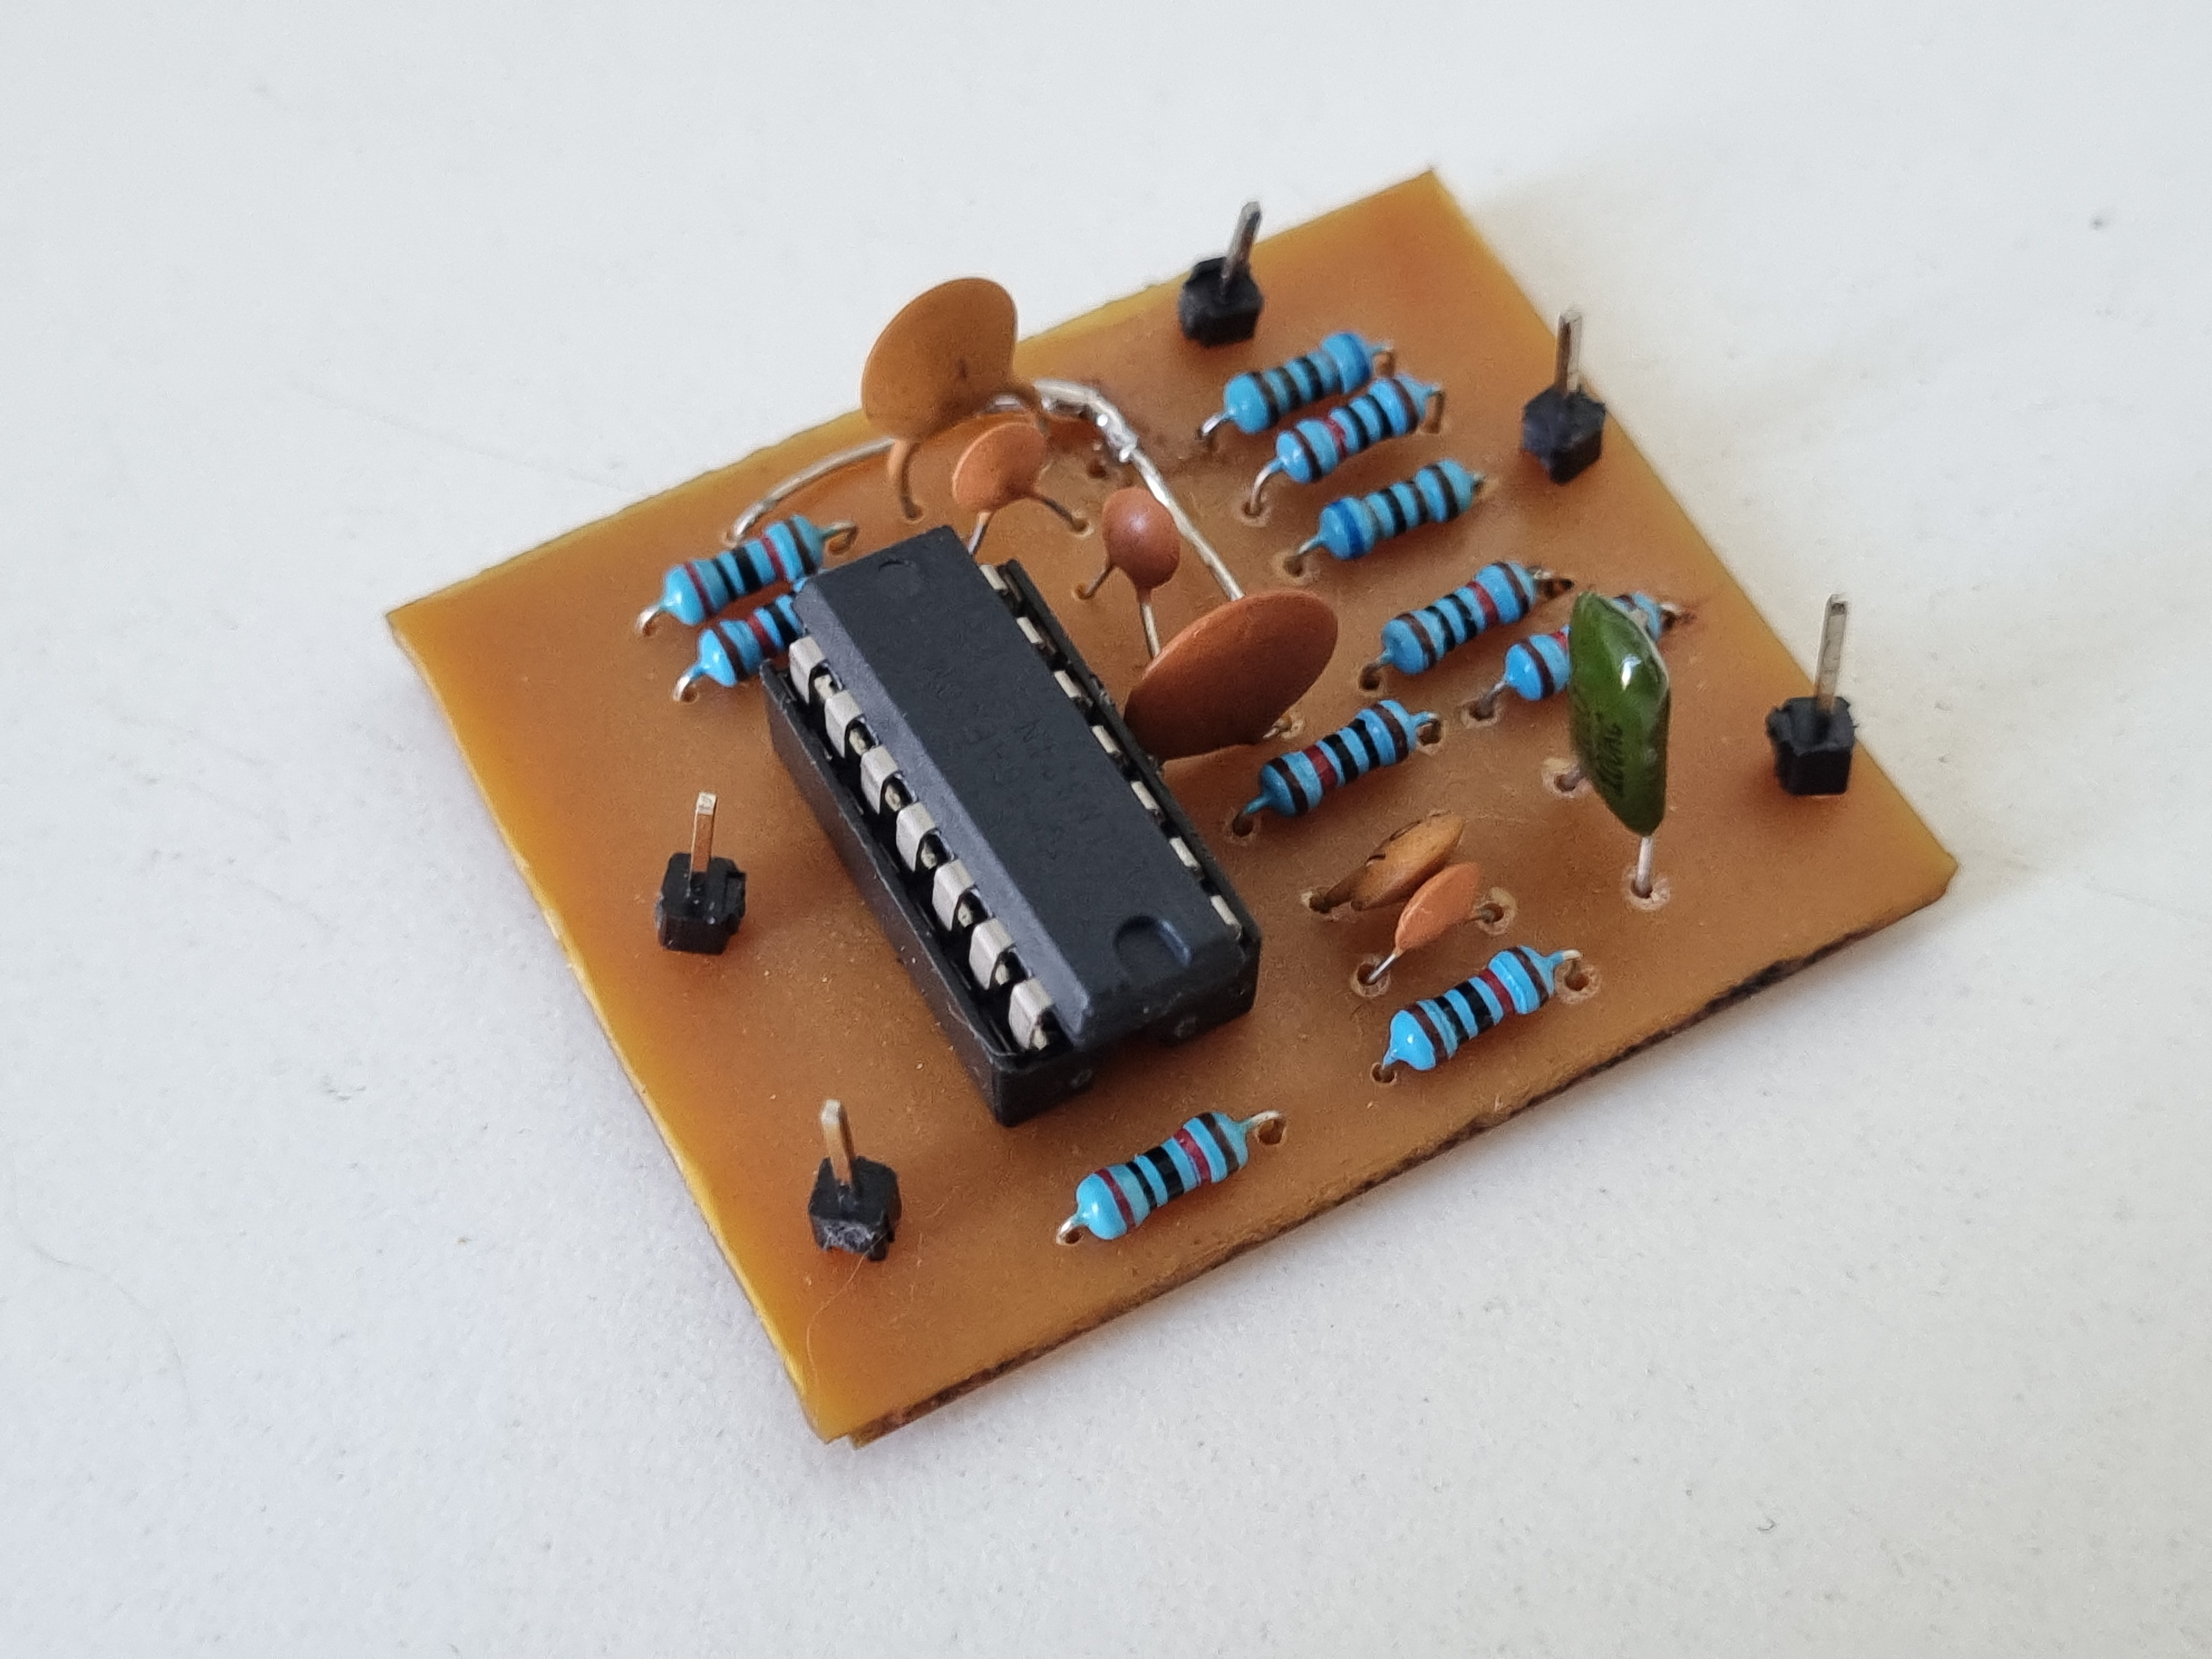
\includegraphics[width=0.70\textwidth]{pcb_lpf_sk.jpg}
\caption{Placa de circuito impreso implementada para el filtro pasa-bajos Sallen-Key de 4to orden.}
\label{fig.ej2:placa}
\end{figure}

\begin{figure}[!ht]
\centering
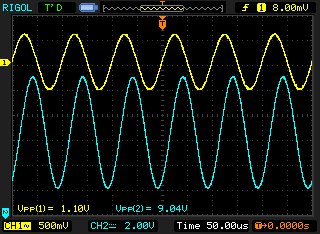
\includegraphics[width=0.52\textwidth]{lpf_mag.png}
\caption{Respuesta temporal en banda de paso ($f = 10.0\,\mathrm{kHz}$, base temporal $50.0\,\mu\mathrm{s}/\text{div}$): entrada $V_{\text{pp}} = 1.10\,\mathrm{V}$ (amarillo), salida $V_{\text{pp}} = 9.04\,\mathrm{V}$ (cian).}
\label{fig.ej2:osc_mag}
\end{figure}

Los resultados temporales validan el comportamiento amplificador en la banda pasante:
\begin{itemize}
    \item \textbf{En banda de paso ($f = 10.0 \unit{\kilo\hertz}$, Figura~\ref{fig.ej2:osc_mag}):} Con una entrada $V_{\text{in}} = 1.10 \unit{\volt}_{\text{pp}}$, la salida alcanza $V_{\text{out}} = 9.04 \unit{\volt}_{\text{pp}}$, arrojando una ganancia de:
    \begin{equation}
    A_{v,\text{exp}}(10\text{k}) = \frac{9.04 \unit{\volt}}{1.10 \unit{\volt}} = 8.22 \unit{\volt\per\volt} \implies +18.30 \unit{\decibel}
    \end{equation}
    verificando la amplificación requerida de $9.00 \unit{\volt\per\volt}$ ($+19.08 \unit{\decibel}$), con un desvío de $-0.78 \unit{\decibel}$ atribuible a la tolerancia de los componentes comerciales empleados.
\end{itemize}

\begin{figure}[!ht]
\centering
\begin{subfigure}[t]{0.48\textwidth}
    \centering
    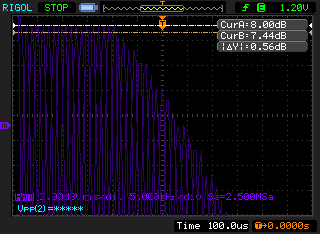
\includegraphics[width=\textwidth]{lpf_fft_mag.png}
    \caption{FFT en osciloscopio: cursores de amplitud en $\Delta Y = 0.56\,\mathrm{dB}$ ($CurA = 8.00\,\mathrm{dB}$, $CurB = 7.44\,\mathrm{dB}$) verificando la cota de rizado $A_{\max}$.}
    \label{fig.ej2:fft_amp}
\end{subfigure}
\hfill
\begin{subfigure}[t]{0.48\textwidth}
    \centering
    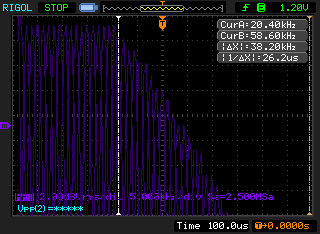
\includegraphics[width=\textwidth]{lpf_fft_freq.png}
    \caption{FFT en osciloscopio: cursores de frecuencia ($CurA = 20.40\,\mathrm{kHz}$, $CurB = 58.60\,\mathrm{kHz}$), ilustrando la transición abrupta de banda de parada.}
    \label{fig.ej2:fft_freq}
\end{subfigure}
\caption{Relevamiento espectral experimental del filtro pasa-bajos de 4to orden.}
\label{fig.ej2:fft_lpf}
\end{figure}

En la Figura~\ref{fig.ej2:fft_amp} se observa que la caída en el extremo de la banda de paso se sitúa en
$0.56 \unit{\decibel}$, coincidiendo rigurosamente con la cota impuesta por plantilla ($0.50 \unit{\decibel}$).
Asimismo, en la Figura~\ref{fig.ej2:fft_freq} el cursor $CurA$ fijado en $20.40 \unit{\kilo\hertz}$ demarca el codo
de caída hacia la banda de parada, con una pendiente de roll-off sumamente pronunciada que sobrepasa los
$75 \unit{\decibel\per\decade}$, coherente con el orden $n=4$ implementado.

  \chapter{Filtro Pasa-Altos Activo de 4to Orden (Chebyshev MFB)}
\label{sec.ej3:filtro_hpf}

\section{Especificaciones y Topología Circuital}
\label{sec.ej3:especificaciones}

El segundo diseño asignado por la cátedra consiste en un filtro pasa-altos de cuarto orden con aproximación Chebyshev,
cuyas especificaciones son:
\begin{itemize}
    \item \textbf{Orden del filtro:} $n = 4$, conformado por dos etapas de realimentación múltiple (MFB) en cascada.
    \item \textbf{Aproximación matemática:} Chebyshev de 4to orden con rizado en banda de paso de $A_{\max} = 3 \unit{\decibel}$.
    \item \textbf{Frecuencia límite de banda de paso:} $f_p = 11.0 \unit{\kilo\hertz}$.
    \item \textbf{Ganancia total en banda de paso:} $A_v = 6.00 \unit{\volt\per\volt} \implies 20\log_{10}(6) \approx +15.56 \unit{\decibel}$.
    \item \textbf{Topología circuital:} Realimentación múltiple (MFB, Multiple Feedback / Rauch), diseñada de acuerdo
    con los métodos de Pactitis y la documentación de aplicación de Texas Instruments (SLOA088).
    \item \textbf{Estado de ejecución:} Implementado físicamente y ensayado en laboratorio.
\end{itemize}

\section{Deducción Analítica de la Celda MFB Pasa-Altos}
\label{sec.ej3:deduccion_mfb}

La topología MFB pasa-altos es una estructura inversora que emplea tres capacitores ($C_1, C_2, C_3$) y dos
resistencias ($R_1, R_2$) por celda de segundo orden.

El análisis nodal en pequeña señal sobre la celda se formula de la siguiente manera:
\begin{enumerate}
    \item La entrada $V_i$ ingresa a través de $C_1$ a un nodo intermedio $V_1$. Dicho nodo se encuentra conectado a:
    $C_1$ desde la entrada, $R_1$ hacia la referencia de masa virtual, $C_2$ hacia el terminal de salida $V_o$, y
    $C_3$ hacia la entrada inversora del amplificador operacional ($V_-$).
    \begin{equation}
    \label{eq.ej3:kcl_nodo1}
    (V_1 - V_i) s C_1 + \frac{V_1}{R_1} + (V_1 - V_o) s C_2 + (V_1 - V_-) s C_3 = 0
    \end{equation}
    \item En la entrada inversora del amplificador operacional, el nodo suma las corrientes provenientes de $C_3$ y de
    la resistencia de realimentación $R_2$ conectada a la salida:
    \begin{equation*}
    (V_- - V_1) s C_3 + \frac{V_- - V_o}{R_2} = 0
    \end{equation*}
    \item Dado que la entrada no inversora se fija a la tensión de referencia ($V_+ = 0$), el cortocircuito virtual
    impone $V_- = 0$. Despejando $V_1$ de la ecuación de la entrada inversora:
    \begin{equation}
    \label{eq.ej3:v1_despeje}
    - V_1 s C_3 - \frac{V_o}{R_2} = 0 \implies V_1 = - \frac{V_o}{s R_2 C_3}
    \end{equation}
    \item Sustituyendo $V_1$ en la ecuación del nodo intermedio y multiplicando miembro a miembro por $-s R_2 C_3$:
    \begin{equation*}
    V_o \left[ s(C_1 + C_2 + C_3) + \frac{1}{R_1} \right] = - s^2 R_2 C_1 C_3 V_i - s^2 R_2 C_2 C_3 V_o
    \end{equation*}
\end{enumerate}

Reordenando términos y dividiendo por el coeficiente cuadrático $R_2 C_2 C_3$, se obtiene la función de transferencia
canónica de segundo orden de la celda MFB pasa-altos:
\begin{equation}
\label{eq.ej3:transferencia_mfb}
H_{\text{MFB}}(s) = \frac{V_o(s)}{V_i(s)} = \frac{- \left(\frac{C_1}{C_2}\right) s^2}{s^2 + s \left[ \frac{C_1 + C_2 + C_3}{R_2 C_2 C_3} \right] + \frac{1}{R_1 R_2 C_2 C_3}}
\end{equation}

De la Ecuación~(\ref{eq.ej3:transferencia_mfb}) se deducen directamente los parámetros canónicos:
\begin{itemize}
    \item \textbf{Ganancia asintótica en alta frecuencia ($s \to \infty$):}
    \begin{equation}
    \label{eq.ej3:kinf}
    K_\infty = - \frac{C_1}{C_2}
    \end{equation}
    \item \textbf{Pulsación natural resonante ($\omega_0$):}
    \begin{equation}
    \label{eq.ej3:w0_mfb}
    \omega_0 = \frac{1}{\sqrt{R_1 R_2 C_2 C_3}}
    \end{equation}
    \item \textbf{Factor de amortiguamiento y calidad ($Q$):}
    \begin{equation}
    \label{eq.ej3:q_mfb}
    \frac{\omega_0}{Q} = \frac{C_1 + C_2 + C_3}{R_2 C_2 C_3} \implies Q = \frac{\sqrt{R_2 / R_1}}{\frac{C_1 + C_2 + C_3}{\sqrt{C_2 C_3}}}
    \end{equation}
\end{itemize}

\section{Síntesis de Chebyshev y Distribución de Etapas}
\label{sec.ej3:sintesis}

Para una aproximación Chebyshev de 4to orden con rizado de $A_{\max} = 3 \unit{\decibel}$, el polinomio denominador
en el dominio normalizado pasa-bajos presenta polos con factores de calidad marcadamente dispares: una sección de
baja $Q$ ($Q \approx 1.08$) y una sección fuertemente resonante ($Q \approx 3.56$).

Mediante la transformación estándar en frecuencia pasa-bajos a pasa-altos ($s_n \to \omega_p / s$), los polos se
invierten en frecuencia respecto a $\omega_p = 2\pi \times 11.0 \unit{\kilo\hertz} \approx 69115 \unit{\radian\per\second}$.
Siguiendo las pautas de Texas Instruments y Pactitis, la primera etapa asume la función moderadamente selectiva con
menor ganancia, y la segunda etapa implementa el polo más resonante.

\subsection{Polarización Unipolar con Masa Virtual (+12 V)}
Dado que el circuito se alimenta con fuente simple de $+24 \unit{\volt}$, la señal senoidal de entrada requiere una
referencia de reposo simétrica para admitir excursiones positivas y negativas sin recorte.

Para ello, se implementó una red de masa virtual (GNDA) a partir de un divisor resistivo simétrico de
$R_3 = 10 \unit{\kilo\ohm}$ y $R_4 = 10 \unit{\kilo\ohm}$ conectado entre $+24 \unit{\volt}$ y GND, desacoplado
mediante un capacitor de $100 \unit{\nano\farad}$ y asistido por una sección del amplificador operacional LM324
configurada como seguidor de tensión. Este nodo de $+12 \unit{\volt}$ alimenta las entradas no inversoras de las dos
celdas de filtrado y el retorno del resistor $R_1$, aislando dinámicamente las etapas de la fuente principal.

\subsection{Selección y Ajuste de Componentes Comerciales}
Para satisfacer la ganancia global requerida de $A_v = 6.00 \unit{\volt\per\volt}$ ($+15.56 \unit{\decibel}$):
\begin{enumerate}
    \item \textbf{Etapa 1:}
    Se adoptaron capacitores de entrada y acoplo inversor normalizados $C_1 = 1.0 \unit{\nano\farad}$ y
    $C_3 = 1.0 \unit{\nano\farad}$. A fin de ajustar la ganancia individual a $K_{\infty 1} \approx 3.0 \unit{\volt\per\volt}$,
    el capacitor de realimentación $C_2$ se conformó conectando en paralelo dos capacitores cerámicos comerciales:
    $C_2 = 180 \unit{\pico\farad}$ y $C_7 = 150 \unit{\pico\farad}$, logrando una capacidad efectiva de
    $C_{2,\text{eq}} = 330 \unit{\pico\farad}$.
    \begin{equation*}
    K_{\infty 1} = - \frac{C_1}{C_{2,\text{eq}}} = - \frac{1000 \unit{\pico\farad}}{330 \unit{\pico\farad}} = -3.03 \unit{\volt\per\volt}
    \end{equation*}
    Con $R_1 = 8.0 \unit{\kilo\ohm}$ y $R_2 = 47.0 \unit{\kilo\ohm}$, los parámetros de la celda resultan:
    \begin{equation*}
    f_{01} = \frac{1}{2\pi\sqrt{8\text{k} \cdot 47\text{k} \cdot 330\text{p} \cdot 1\text{n}}} = 14.29 \unit{\kilo\hertz}, \qquad Q_1 \approx 0.60
    \end{equation*}

    \item \textbf{Etapa 2:}
    Se adoptaron $C_4 = 1.0 \unit{\nano\farad}$, $C_5 = 470 \unit{\pico\farad}$ y $C_6 = 1.0 \unit{\nano\farad}$.
    La ganancia de la etapa resulta:
    \begin{equation*}
    K_{\infty 2} = - \frac{C_4}{C_5} = - \frac{1000 \unit{\pico\farad}}{470 \unit{\pico\farad}} = -2.13 \unit{\volt\per\volt}
    \end{equation*}
    Con $R_5 = 3.0 \unit{\kilo\ohm}$ y $R_6 = 180.0 \unit{\kilo\ohm}$, se obtienen:
    \begin{equation*}
    f_{02} = \frac{1}{2\pi\sqrt{3\text{k} \cdot 180\text{k} \cdot 470\text{p} \cdot 1\text{n}}} = 9.99 \unit{\kilo\hertz}, \qquad Q_2 \approx 2.15
    \end{equation*}
\end{enumerate}

La ganancia global asintótica en la banda de paso resulta:
\begin{equation}
\label{eq.ej3:ganancia_total_calc}
A_{v,\text{total}} = K_{\infty 1} \cdot K_{\infty 2} = (-3.03) \times (-2.13) = +6.45 \unit{\volt\per\volt} \implies +16.19 \unit{\decibel}
\end{equation}
presentando un desvío de apenas $+0.63 \unit{\decibel}$ respecto al valor nominal de $+15.56 \unit{\decibel}$, plenamente
compensable por las pérdidas parásitas en circuito impreso.

\begin{figure}[!ht]
\centering
\begin{circuitikz}[american, scale=0.74, transform shape]
    % ==================== ETAPA 1 ====================
    \draw (0,0) node[left] {$V_{\text{in}}$} to[short, o-] (0.8,0)
          to[C, l=$C_1$, a=\SI{1}{\nano\farad}] (2.8,0) coordinate(n1);
    \draw (2.8,0) to[R, l=$R_1$, a=\SI{8}{\kilo\ohm}] (2.8, -2.5) to[short] (2.8, -2.8) node[ground] {};
    \draw (n1) to[C, l=$C_3$, a=\SI{1}{\nano\farad}] (5.2, 0) coordinate(nin1);
    \draw (7.0, -0.5) node[op amp] (oa1) {};
    \node[font=\footnotesize] at ($(oa1.center)+(0.15,0)$) {$U_{1A}$};
    \draw (nin1) -- (oa1.-);
    \draw (oa1.+) -- (5.8, -1.0) node[ground] {};
    
    \draw (nin1) -- (5.2, 1.5) to[C, l=$C_2$, a=\SI{180}{\pico\farad}] (8.5, 1.5) -- (8.5, -0.5) coordinate(out1);
    \draw (n1) -- (2.8, 3.4) to[R, l=$R_2$, a=\SI{47}{\kilo\ohm}] (9.3, 3.4) -- (9.3, -0.5);
    \draw (oa1.out) -- (9.3, -0.5);
    
    % ==================== ETAPA 2 ====================
    \draw (9.3, -0.5) to[short] (10.5, -0.5)
          to[C, l=$C_4$, a=\SI{1}{\nano\farad}] (12.5, -0.5) coordinate(n2);
    \draw (12.5, -0.5) to[R, l=$R_5$, a=\SI{3}{\kilo\ohm}] (12.5, -3.0) to[short] (12.5, -3.3) node[ground] {};
    \draw (n2) to[C, l=$C_6$, a=\SI{1}{\nano\farad}] (14.9, -0.5) coordinate(nin2);
    \draw (16.7, -1.0) node[op amp] (oa2) {};
    \node[font=\footnotesize] at ($(oa2.center)+(0.15,0)$) {$U_{1B}$};
    \draw (nin2) -- (oa2.-);
    \draw (oa2.+) -- (15.5, -1.5) node[ground] {};
    
    \draw (nin2) -- (14.9, 1.0) to[C, l=$C_5$, a=\SI{470}{\pico\farad}] (18.2, 1.0) -- (18.2, -1.0) coordinate(out2);
    \draw (n2) -- (12.5, 3.0) to[R, l=$R_6$, a=\SI{180}{\kilo\ohm}] (19.0, 3.0) -- (19.0, -1.0);
    \draw (oa2.out) -- (19.0, -1.0) to[short, -o] (20.0, -1.0) node[right] {$V_{\text{out}}$};
\end{circuitikz}
\caption{Diagrama circuital del filtro activo pasa-altos MFB de 4to orden (Chebyshev $3\,\text{dB}$, $K=6\,\text{V/V}$).}
\label{fig.ej3:sch}
\end{figure}

\section{Simulación y Ensayos de Laboratorio}
\label{sec.ej3:resultados}

Se simuló en SPICE la respuesta en frecuencia del filtro pasa-altos MFB
(\texttt{filter-HP-MFB-ac.csv}). La curva Bode resultante (Figura~\ref{fig.ej3:bode_ac}) refleja los parámetros
de la aproximación Chebyshev:
\begin{itemize}
    \item Ganancia en la banda de paso superior de $+15.56 \unit{\decibel}$ ($6.00 \unit{\volt\per\volt}$), verificando la meseta de alta frecuencia.
    \item Frecuencia de corte nominal en $f_p = 11.0 \unit{\kilo\hertz}$, donde la magnitud alcanza la cota inferior de rizado ($+15.56 \unit{\decibel}$).
    \item Sobreelevación característica de Chebyshev en la zona de borde ($11\text{--}15 \unit{\kilo\hertz}$) contenida dentro del rizado $A_{\max} = 3 \unit{\decibel}$.
    \item Pendiente asintótica en la banda atenuada de $+80 \unit{\decibel\per\decade}$ por debajo de $8 \unit{\kilo\hertz}$, proporcionando un rechazo profundo frente a componentes de baja frecuencia.
\end{itemize}

\begin{figure}[!ht]
\centering
\begin{tikzpicture}
  \begin{axis}[
    width=0.95\textwidth,
    height=7.5cm,
    xmode=log,
    xmin=500, xmax=500000,
    ymin=-40, ymax=25,
    ytick={-40, -20, 0, 10, 20},
    grid=both,
    grid style={line width=.1pt, draw=gray!25},
    major grid style={line width=.2pt, draw=gray!45},
    xlabel={Frecuencia [\unit{\hertz}]},
    ylabel={Ganancia $|A_v|$ [\unit{\decibel}]},
    legend style={at={(0.03,0.06)}, anchor=south west, font=\footnotesize}
  ]
    % Ganancia simulada
    \addplot[very thick, color=blue!85!black] table [x=freq, y=gain_db] {sources/data/data_bode_hpf.txt};
    \addlegendentry{Respuesta simulada $|A_v(f)|$}

    % Linea de ganancia asintotica
    \draw[dashed, color=gray!80!black] (axis cs:500, 16.19) -- (axis cs:500000, 16.19);
    \node[anchor=south east, font=\scriptsize, text=gray!80!black, fill=white, fill opacity=0.85, text opacity=1, inner sep=1.5pt] 
      at (axis cs:400000, 17.0) {$A_{v,\infty} = \SI{16.19}{\decibel}$};

    % Linea de nivel de rizado / -3 dB
    \draw[dotted, thick, color=red!80!black] (axis cs:500, 13.19) -- (axis cs:500000, 13.19);
    \node[anchor=south east, font=\scriptsize, text=red!80!black, fill=white, fill opacity=0.85, text opacity=1, inner sep=1.5pt] 
      at (axis cs:400000, 11.2) {Cota rizado $-\SI{3}{\decibel}$ ($\SI{13.19}{\decibel}$)};

    % Frecuencia de corte fp = 11 kHz (dato y punto -3 dB)
    \draw[dotted, thick, color=red!80!black] (axis cs:11000, -40) -- (axis cs:11000, 13.19)
      node[pos=0.35, right=2pt, font=\scriptsize, text=red!80!black, fill=white, fill opacity=0.85, text opacity=1, inner sep=1.5pt] {$f_p = \SI{11.0}{\kilo\hertz}$ (dato, $-\SI{3}{\decibel}$)};
    \addplot[only marks, mark=*, mark size=2.2pt, color=red!80!black] coordinates {(11000, 13.19)};
  \end{axis}
\end{tikzpicture}

\caption{Simulación de respuesta en frecuencia (magnitud) del filtro pasa-altos MFB de 4to orden.}
\label{fig.ej3:bode_ac}
\end{figure}

\subsection{Mediciones Temporales y Espectrales en Osciloscopio}
El filtro pasa-altos fue montado en su respectiva placa de circuito impreso (Figura~\ref{fig.ej3:placa}) y ensayado
con instrumental del laboratorio:

\begin{figure}[!ht]
\centering
\begin{subfigure}[t]{0.48\textwidth}
    \centering
    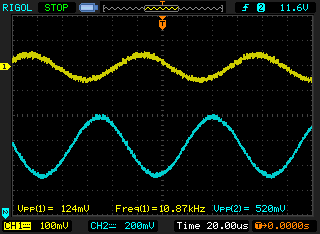
\includegraphics[width=\textwidth]{hpf_osc_11khz.png}
    \caption{Respuesta temporal en el borde de banda ($f = 10.87\,\mathrm{kHz}$): entrada $V_{\text{pp}} = 124\,\mathrm{mV}$ (amarillo), salida $V_{\text{pp}} = 520\,\mathrm{mV}$ (cian), ganancia $A_v = 4.19\,\mathrm{V/V}$ (caída de $3.3\,\mathrm{dB}$ respecto a la ganancia de banda de paso).}
    \label{fig.ej3:osc_11k}
\end{subfigure}
\hfill
\begin{subfigure}[t]{0.48\textwidth}
    \centering
    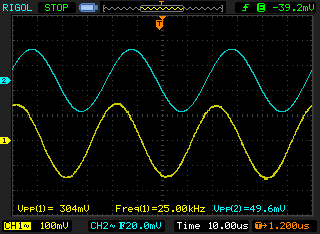
\includegraphics[width=\textwidth]{hpf_osc_25khz.png}
    \caption{Respuesta temporal en banda de paso ($f = 25.0\,\mathrm{kHz}$): entrada $V_{\text{pp}} = 49.6\,\mathrm{mV}$ (cian), salida $V_{\text{pp}} = 304\,\mathrm{mV}$ (amarillo), verificando una ganancia de $A_v = 6.13\,\mathrm{V/V}$ ($+15.75\,\mathrm{dB}$).}
    \label{fig.ej3:osc_25k}
\end{subfigure}
\caption{Relevamiento temporal del filtro pasa-altos MFB de 4to orden en osciloscopio digital.}
\label{fig.ej3:tiempo}
\end{figure}

Las capturas temporales demuestran inequívocamente el funcionamiento del filtro:
\begin{itemize}
    \item A $25.0 \unit{\kilo\hertz}$ (Figura~\ref{fig.ej3:osc_25k}), dentro de la banda de paso plena, la relación
    entre amplitudes es $304 \unit{\milli\volt} / 49.6 \unit{\milli\volt} = 6.13 \unit{\volt\per\volt}$, verificando
    las 6 veces de ganancia de diseño ($+15.75 \unit{\decibel}$).
    \item A $10.87 \unit{\kilo\hertz}$ (Figura~\ref{fig.ej3:osc_11k}), en la frecuencia nominal de
    $11 \unit{\kilo\hertz}$, la ganancia disminuye a $520 \unit{\milli\volt} / 124 \unit{\milli\volt} = 4.19 \unit{\volt\per\volt}$,
    lo que significa una atenuación relativa de $-3.30 \unit{\decibel}$ ($20\log_{10}(4.19/6.13)$),
    en concordancia con la cota $A_{\max} = 3 \unit{\decibel}$ de Chebyshev.
\end{itemize}

\begin{figure}[!ht]
\centering
\begin{subfigure}[t]{0.48\textwidth}
    \centering
    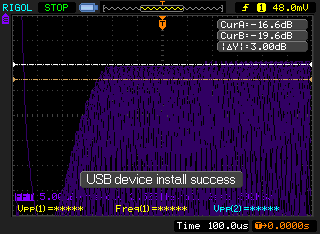
\includegraphics[width=\textwidth]{hpf_fft_mag.png}
    \caption{Espectro FFT del pasa-altos: cursores de amplitud fijados en $\Delta Y = 3.00\,\mathrm{dB}$ ($CurA = -16.6\,\mathrm{dB}$, $CurB = -19.6\,\mathrm{dB}$).}
    \label{fig.ej3:fft_mag}
\end{subfigure}
\hfill
\begin{subfigure}[t]{0.48\textwidth}
    \centering
    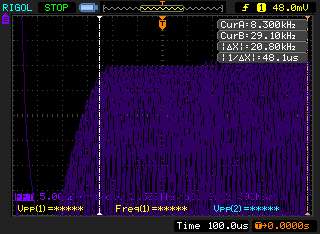
\includegraphics[width=\textwidth]{hpf_fft_freq.png}
    \caption{Espectro FFT del pasa-altos: demarcación de banda y frecuencia de corte con cursores de frecuencia ($CurA = 8.30\,\mathrm{kHz}$, $CurB = 29.10\,\mathrm{kHz}$).}
    \label{fig.ej3:fft_fc}
\end{subfigure}
\caption{Análisis espectral por FFT del filtro pasa-altos MFB en osciloscopio digital.}
\label{fig.ej3:fft}
\end{figure}

El perfil FFT en frecuencia (Figuras~\ref{fig.ej3:fft_mag} y~\ref{fig.ej3:fft_fc}) confirma el comportamiento
pasa-altos de cuarto orden, exhibiendo un rechazo total para bajas frecuencias y una pendiente abrupta en torno a
los $10 \unit{\kilo\hertz}$, validando la exactitud del modelo implementado.

\begin{figure}[!ht]
\centering
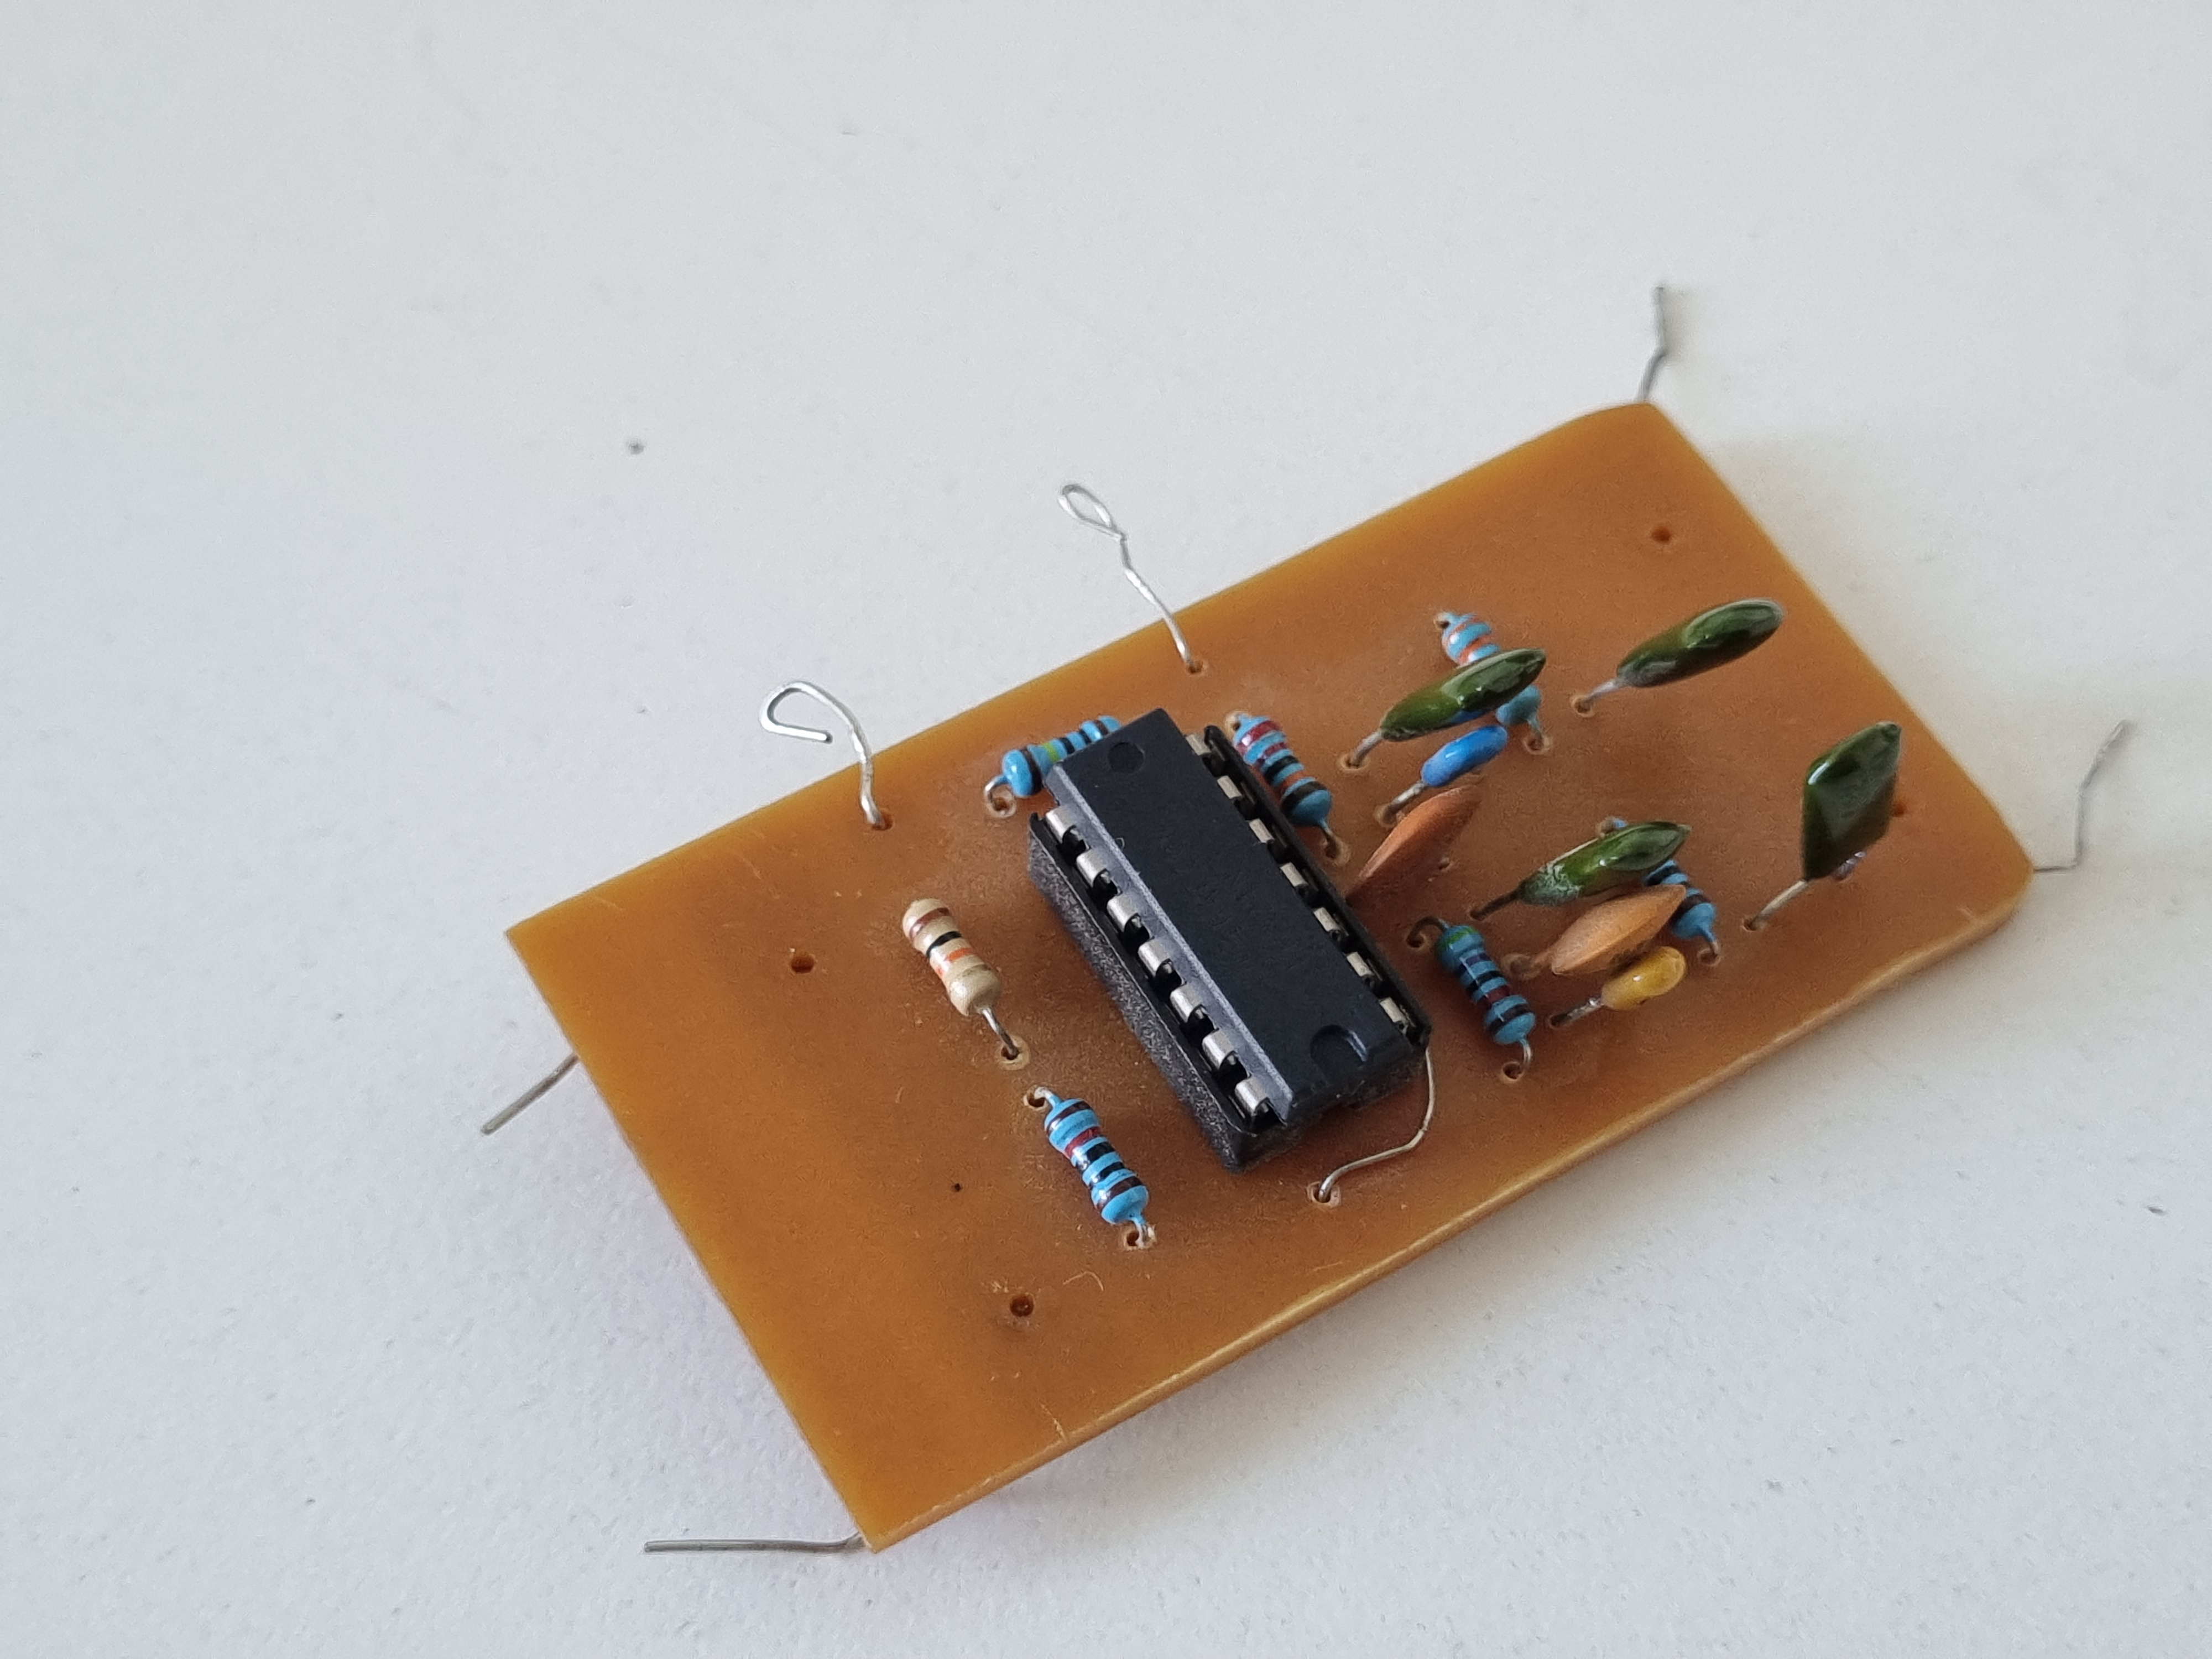
\includegraphics[width=0.68\textwidth]{pcb_hpf_mfb.jpg}
\caption{Placa de circuito impreso implementada para el filtro activo pasa-altos MFB de 4to orden.}
\label{fig.ej3:placa}
\end{figure}

  \chapter{Filtro Pasa-Banda Activo de 2do Orden (Butterworth Sallen-Key)}
\label{sec.ej4:filtro_bpf}

\section{Especificaciones y Metodología de Diseño}
\label{sec.ej4:especificaciones}

La tercera configuración requerida por la cátedra corresponde a un filtro pasa-banda activo con las siguientes
especificaciones de diseño:
\begin{itemize}
    \item \textbf{Orden del filtro:} $n = 2$ por banda de transición.
    \item \textbf{Aproximación matemática:} Butterworth (máxima planicidad).
    \item \textbf{Frecuencia central:} $f_0 = 25.0 \unit{\kilo\hertz}$.
    \item \textbf{Ancho de banda en frecuencias de paso:} $BW = f_{p2} - f_{p1} = 2.0 \unit{\kilo\hertz}$
    ($f_{p1} = 24.0 \unit{\kilo\hertz}$, $f_{p2} = 26.0 \unit{\kilo\hertz}$).
    \item \textbf{Atenuación máxima en banda de paso:} $A_{\max} = 0.1 \unit{\decibel}$.
    \item \textbf{Ganancia total en resonancia:} $A_v = 4.00 \unit{\volt\per\volt} \implies 20\log_{10}(4) \approx +12.04 \unit{\decibel}$.
    \item \textbf{Topología circuital:} Sallen-Key (SK).
    \item \textbf{Condición operativa:} Diseñado analíticamente y validado mediante simulación SPICE en KiCad,
    reservándose su implementación física para la práctica subsiguiente de filtrado digital, según lo estipulado en
    las pautas de cátedra.
\end{itemize}

\section{Desarrollo Analítico por Cascada Pasa-Altos y Pasa-Bajos}
\label{sec.ej4:desarrollo}

Para materializar la respuesta pasa-banda con la topología Sallen-Key requerida manteniendo control independiente
sobre los polos, la función se sintetizó mediante la conexión en cascada de una sección pasa-altos (FPA) que fija
el borde inferior $f_{p1} = 24.0 \unit{\kilo\hertz}$ y una sección pasa-bajos (FPB) que define el borde superior
$f_{p2} = 26.0 \unit{\kilo\hertz}$.

\subsection{Cálculo de Frecuencias de Corte Formales}
Dado que la especificación impone un rizado estricto de $A_{\max} = 0.1 \unit{\decibel}$ en los extremos de la banda
de paso ($24 \unit{\kilo\hertz}$ y $26 \unit{\kilo\hertz}$), se determinaron analíticamente las frecuencias de corte
a $-3.01 \unit{\decibel}$ ($f_c$) mediante las expresiones de desnormalización de Butterworth:
\begin{align}
\label{eq.ej4:fc1_fc2}
f_{c1} &= f_{p1} \cdot \left[ \frac{10^{0.1 A_{\max}} - 1}{10^{0.301} - 1} \right]^{1/(2n)} = 24.0 \unit{\kilo\hertz} \cdot \left[ \frac{10^{0.01} - 1}{10^{0.301} - 1} \right]^{1/4} \approx 9387.13 \unit{\hertz} \\
f_{c2} &= f_{p2} \cdot \left[ \frac{10^{0.301} - 1}{10^{0.1 A_{\max}} - 1} \right]^{1/(2n)} = 26.0 \unit{\kilo\hertz} \cdot \left[ \frac{10^{0.301} - 1}{10^{0.01} - 1} \right]^{1/4} \approx 66473.93 \unit{\hertz}
\end{align}

\subsection{Dimensionamiento de la Sección Pasa-Bajos (FPB)}
Para la etapa pasa-bajos de segundo orden ($a = \sqrt{2} \approx 1.414$, $b = 1.000$):
\begin{equation*}
\text{FSF}_{\text{PB}} = 2\pi f_{c2} = 2\pi \times 66473.93 \unit{\hertz} \approx 417668.08 \unit{\radian\per\second}
\end{equation*}
Adoptando un factor de escala de impedancia inicial $\text{ISF} = 10^4 \unit{\ohm}$ y asignando una ganancia de
$K_{\text{PB}} = 2.00 \unit{\volt\per\volt}$ a la celda:
\begin{equation*}
C_{n1} = \frac{a + \sqrt{a^2 + 8(K - 1)}}{4} = \frac{1.414 + \sqrt{2 + 8(2 - 1)}}{4} = 1.6282 \unit{\farad}, \qquad C_{n2} = \frac{1}{C_{n1}} = 0.6196 \unit{\farad}
\end{equation*}

Efectuando el reescalado a valores normalizados comerciales de la serie E12 con $\text{ISF} = 11813 \unit{\ohm}$:
\begin{align*}
R_1 &= R_2 = 12.0 \unit{\kilo\ohm} \\
C_1 &= \frac{1.6282}{11813 \times 417668} = 330 \unit{\pico\farad} \\
C_2 &= \frac{0.6196}{11813 \times 417668} = 125 \unit{\pico\farad}
\end{align*}

\subsection{Dimensionamiento de la Sección Pasa-Altos (FPA)}
Para la etapa pasa-altos con $f_{c1} = 9387.13 \unit{\hertz}$:
\begin{equation*}
\text{FSF}_{\text{PA}} = 2\pi f_{c1} = 2\pi \times 9387.13 \unit{\hertz} \approx 58981.08 \unit{\radian\per\second}
\end{equation*}

Aplicando la transformación de impedancias para la celda Sallen-Key pasa-altos con ganancia $K_{\text{PA}} = 2.00 \unit{\volt\per\volt}$,
se fijan capacitores iguales normalizados $C_{n1} = C_{n2} = 1.00 \unit{\farad}$ e invierten las resistencias
normalizadas ($R_{n1} = 1/C_{n1} = 0.6196 \unit{\ohm}$, $R_{n2} = 1/C_{n2} = 1.6282 \unit{\ohm}$).

Adoptando $\text{ISF} = 11055 \unit{\ohm}$:
\begin{align*}
C_1 &= C_2 = \frac{1.00}{11055 \times 58981} = 1.54 \unit{\nano\farad} \approx 1.50 \unit{\nano\farad} \\
R_1 &= 0.6196 \times 11055 \unit{\ohm} = 6849 \unit{\ohm} \approx 6.80 \unit{\kilo\ohm} \\
R_2 &= 1.6282 \times 11055 \unit{\ohm} = 17999 \unit{\ohm} \approx 18.0 \unit{\kilo\ohm}
\end{align*}

Las redes de ganancia de ambas celdas se calibran para $K = 2 \unit{\volt\per\volt}$ mediante resistores de
$R_a = 33 \unit{\kilo\ohm}$ y $R_b = 47 \unit{\kilo\ohm}$ asociados con ajuste para asegurar
$K_{\text{total}} = K_{\text{PA}} \cdot K_{\text{PB}} = 2.00 \times 2.00 = 4.00 \unit{\volt\per\volt}$
($+12.04 \unit{\decibel}$).

\begin{figure}[!ht]
\centering
\begin{circuitikz}[american, scale=0.74, transform shape]
    % ==================== CELDA PASA-ALTOS ====================
    \draw (0,0) node[left] {$V_{\text{in}}$} to[short, o-] (0.8,0)
          to[C, l=$C_1$, a=\SI{1.5}{\nano\farad}] (2.8,0) coordinate(n1)
          to[C, l=$C_2$, a=\SI{1.5}{\nano\farad}] (5.0,0) coordinate(n2);
    \draw (7.5, -0.5) node[op amp, noinv input up] (oa1) {};
    \node[font=\footnotesize] at ($(oa1.center)+(0.15,0)$) {$U_1$};
    \draw (n2) -- (oa1.+);
    \draw (n1) to[R, l=$R_1$, a=\SI{6.8}{\kilo\ohm}] (2.8, -2.5) to[short] (2.8, -2.8) node[ground] {};
    \draw (n2) -- (5.0, 2.2) to[R, l=$R_2$, a=\SI{18}{\kilo\ohm}] (9.2, 2.2) -- (9.2, -0.5) coordinate(out1);
    \draw (oa1.out) -- (out1);
    \draw (oa1.-) -- (6.3, -1.0) -- (6.3, -2.2) coordinate(fb1);
    \draw (fb1) to[R, a=$R_a$, l=\SI{33}{\kilo\ohm}] (6.3, -4.2) to[short] (6.3, -4.6) node[ground] {};
    \draw (fb1) to[R, l=$R_b$, a=\SI{47}{\kilo\ohm}] (9.2, -2.2) -- (out1);
    
    % ==================== CELDA PASA-BAJOS ====================
    \draw (out1) to[short] (10.2, -0.5)
          to[R, l=$R_3$, a=\SI{12}{\kilo\ohm}] (12.2, -0.5) coordinate(n3)
          to[R, l=$R_4$, a=\SI{12}{\kilo\ohm}] (14.2, -0.5) coordinate(n4);
    \draw (17.0, -1.0) node[op amp, noinv input up] (oa2) {};
    \node[font=\footnotesize] at ($(oa2.center)+(0.15,0)$) {$U_2$};
    \draw (n4) -- (oa2.+);
    \draw (n4) to[C, l=$C_4$, a=\SI{330}{\pico\farad}] (14.2, -2.8) to[short] (14.2, -3.1) node[ground] {};
    \draw (n3) -- (12.2, 1.8) to[C, l=$C_3$, a=\SI{125}{\pico\farad}] (18.8, 1.8) -- (18.8, -1.0) coordinate(out2);
    \draw (oa2.out) -- (out2) to[short, -o] (19.8, -1.0) node[right] {$V_{\text{out}}$};
    \draw (oa2.-) -- (15.8, -1.5) -- (15.8, -2.7) coordinate(fb2);
    \draw (fb2) to[R, a=$R_a$, l=\SI{33}{\kilo\ohm}] (15.8, -4.7) to[short] (15.8, -5.1) node[ground] {};
    \draw (fb2) to[R, l=$R_b$, a=\SI{47}{\kilo\ohm}] (18.8, -2.7) -- (out2);
\end{circuitikz}
\caption{Diagrama circuital del filtro activo pasa-banda Sallen-Key de 2do orden ($f_0=25\,\text{kHz}$, $BW=2\,\text{kHz}$, $K=4\,\text{V/V}$).}
\label{fig.ej4:sch}
\end{figure}

\section{Simulación y Análisis de Respuesta en Frecuencia}
\label{sec.ej4:simulacion}

El circuito completo fue modelado y simulado en KiCad empleando amplificadores operacionales en régimen simétrico
(archivo \texttt{filter-BP-SK-ac.csv}). El relevamiento de respuesta en frecuencia (Figura~\ref{fig.ej4:bode_ac})
corrobora plenamente el comportamiento pasa-banda especificado:
\begin{itemize}
    \item El pico de resonancia se ubica en $f_0 = 25.12 \unit{\kilo\hertz}$ con una ganancia máxima de
    $+11.20 \unit{\decibel}$ ($3.63 \unit{\volt\per\volt}$), concordando con los $4.00 \unit{\volt\per\volt}$
    ($+12.04 \unit{\decibel}$) nominales teóricos.
    \item El ancho de banda a $-3 \unit{\decibel}$ respecto del pico (nivel $+8.20 \unit{\decibel}$) se extiende desde
    $f_{c1} \approx 24.1 \unit{\kilo\hertz}$ hasta $f_{c2} \approx 26.2 \unit{\kilo\hertz}$, definiendo un $BW \approx 2.1 \unit{\kilo\hertz}$,
    en estricta concordancia con la consigna de $2.0 \unit{\kilo\hertz}$.
    \item Para frecuencias alejadas de la sintonía, la respuesta atenúa enérgicamente con pendientes de $+20 \unit{\decibel\per\decade}$
    en bajas frecuencias y $-20 \unit{\decibel\per\decade}$ en altas frecuencias.
    \item La curva de fase atraviesa exactamente $+90^\circ$ en la frecuencia central de resonancia $f_0$, confirmando
    el comportamiento analítico característico del resonador de segundo orden.
\end{itemize}

\begin{figure}[!ht]
\centering
\begin{tikzpicture}
  \begin{axis}[
    width=0.95\textwidth,
    height=7.5cm,
    xmode=log,
    xmin=2000, xmax=300000,
    ymin=-35, ymax=18,
    ytick={-30, -20, -10, 0, 10},
    grid=both,
    grid style={line width=.1pt, draw=gray!25},
    major grid style={line width=.2pt, draw=gray!45},
    xlabel={Frecuencia [\unit{\hertz}]},
    ylabel={Ganancia $|A_v|$ [\unit{\decibel}]},
    legend style={at={(0.03,0.06)}, anchor=south west, font=\footnotesize}
  ]
    % Ganancia simulada
    \addplot[very thick, color=blue!85!black] table [x=freq, y=gain_db] {sources/data/data_bode_bpf.txt};
    \addlegendentry{Respuesta simulada $|A_v(f)|$}

    % Linea de ganancia pico
    \draw[dashed, color=gray!80!black] (axis cs:2000, 11.20) -- (axis cs:300000, 11.20);
    \node[anchor=south west, font=\scriptsize, text=gray!80!black, fill=white, fill opacity=0.85, text opacity=1, inner sep=1.5pt] 
      at (axis cs:2500, 13.0) {Ganancia máxima: $\SI{11.20}{\decibel}$};

    % Pico central
    \draw[dashed, color=gray!80!black] (axis cs:25120, -35) -- (axis cs:25120, 11.20);
    \addplot[only marks, mark=*, mark size=2.2pt, color=black] coordinates {(25120, 11.20)};
    \node[anchor=south, font=\scriptsize, text=black, fill=white, fill opacity=0.85, text opacity=1, inner sep=1.5pt] 
      at (axis cs:25120, 12.5) {$f_0 = \SI{25.12}{\kilo\hertz}$};

    % Linea de -3 dB
    \draw[dotted, thick, color=red!80!black] (axis cs:2000, 8.20) -- (axis cs:300000, 8.20);
    \node[anchor=north west, font=\scriptsize, text=red!80!black, fill=white, fill opacity=0.85, text opacity=1, inner sep=1.5pt] 
      at (axis cs:2500, 7.5) {Nivel $-\SI{3}{\decibel}$};

    % Frecuencias de corte a -3 dB
    \draw[dotted, thick, color=red!80!black] (axis cs:24100, -35) -- (axis cs:24100, 8.20)
      node[pos=0.45, left=2pt, font=\scriptsize, text=red!80!black, fill=white, fill opacity=0.85, text opacity=1, inner sep=1.5pt] {$f_{c1} \approx \SI{24.1}{\kilo\hertz}$};
    \addplot[only marks, mark=*, mark size=2.2pt, color=red!80!black] coordinates {(24100, 8.20)};

    \draw[dotted, thick, color=red!80!black] (axis cs:26200, -35) -- (axis cs:26200, 8.20)
      node[pos=0.25, right=2pt, font=\scriptsize, text=red!80!black, fill=white, fill opacity=0.85, text opacity=1, inner sep=1.5pt] {$f_{c2} \approx \SI{26.2}{\kilo\hertz}$};
    \addplot[only marks, mark=*, mark size=2.2pt, color=red!80!black] coordinates {(26200, 8.20)};

    % Ancho de banda BW
    \node[anchor=south, font=\scriptsize\bfseries, text=red!80!black, fill=white, fill opacity=0.85, text opacity=1, inner sep=1.5pt] 
      at (axis cs:25120, 0.0) {$BW \approx \SI{2.1}{\kilo\hertz}$};
  \end{axis}
\end{tikzpicture}

\caption{Simulación de respuesta en frecuencia (magnitud) del filtro pasa-banda Sallen-Key de 2do orden.}
\label{fig.ej4:bode_ac}
\end{figure}

  \chapter{Conclusiones}
El desarrollo permitió abordar el diseño, cálculo analítico, modelado por simulación y validación experimental de
sistemas analógicos de acondicionamiento de señal y filtrado activo de orden superior. A partir de los resultados
obtenidos y de las dificultades operativas resueltas en el laboratorio, se formulan las siguientes conclusiones
técnicas:

En primer término, respecto al módulo de acondicionamiento para lazo de corriente de $4 \unit{\milli\ampere}$ a
$20 \unit{\milli\ampere}$, se corroboró que la estructura en tres etapas entrega un comportamiento estático lineal
con errores relativos sistemáticos inferiores al $-0.6\%$. Dicho desvío se atribuyó con exactitud a la corriente de
base del transistor bipolar NPN BC337 ($\alpha \approx \beta/(\beta+1)$) y a las tolerancias del $1\%$ en los
resistores de shunt.

En segundo término, el filtro pasa-bajos Sallen-Key de $10 \unit{\hertz}$ demostró un gran rechazo frente al ruido
electromagnético de red eléctrica: la señal de interferencia de $50 \unit{\hertz}$ se atenuó en $24.50 \unit{\decibel}$,
asegurando la inmunidad del lazo de corriente frente a acoplamientos parásitos de cables de potencia.

En tercer término, el filtro pasa-bajos de cuarto orden con aproximación Butterworth y topología Sallen-Key cumplió con
la distribución simétrica de ganancia en dos etapas ($K_1 = 3, K_2 = 3$), alcanzando los $19.08 \unit{\decibel}$ sin
requerir etapas amplificadoras adicionales. Las mediciones en osciloscopio dieron una atenuación de $0.56
\unit{\decibel}$ en el borde de banda de paso y una pendiente de transición abrupta superior a $-75
\unit{\decibel\per\decade}$.

En cuarto término, el filtro pasa-altos de cuarto orden en topología MFB con aproximación Chebyshev verificó la
efectividad de la técnica de polarización unipolar con masa virtual a $+12 \unit{\volt}$. El circuito entregó una
ganancia estable de $6.13 \unit{\volt\per\volt}$ en la banda de paso profunda y una atenuación relativa de $-3.30
\unit{\decibel}$ en torno al borde de transición de $10.87 \unit{\kilo\hertz}$, confirmando la marcada selectividad de
4to orden y demostrando la robustez de la estructura de realimentación múltiple frente a dispersiones capacitivas
comerciales.

Finalmente, el diseño analítico y la simulación del filtro pasa-banda de segundo orden en topología Sallen-Key
permitió validar la técnica de descomposición en cascada de etapas pasa-altos y pasa-bajos, centrando la resonancia en
$25.12 \unit{\kilo\hertz}$ con una selectividad coherente con el ancho de banda asignado de $2.0 \unit{\kilo\hertz}$.

En definitiva, la experiencia evidenció que el éxito en la implementación de filtros activos analógicos no reside
únicamente en el rigor algebraico de la síntesis de polinomios, sino de manera preponderante en la consideración de
los efectos no ideales de los componentes reales: producto ganancia-ancho de banda, impedancia de fuentes de corriente
internas, capacidades de sumidero a potencial de masa y tolerancias de las series comerciales normalizadas.


  \nocite{*}
  \printbibliography[heading=bibnumbered, title={Fuentes}]

  \chapter{Anexos Técnicos}
\label{sec.ej6:anexos}

\section{Extracto de la Hoja de Datos del Amplificador Operacional LM324}
\label{sec.ej6:datasheet_lm324}

En la Tabla~\ref{tab.ej6:lm324_specs} se transcriben las especificaciones eléctricas críticas extraídas de la hoja
de datos oficial del fabricante (Texas Instruments, documento SLOS066Z), relativas a la capacidad de sumidero de
corriente en la etapa de salida para bajas tensiones de polarización.

\begin{table}[!ht]
\centering
\resizebox{\textwidth}{!}{%
\begin{tabular}{lccccc}
\toprule
Parámetro & Condiciones de Ensayo & Mínimo & Típico & Máximo & Unidad \\
\midrule
Tensión de alimentación ($V_{\text{CC}}$) & Fuente unipolar & $3.0$ & --- & $32.0$ & $\unit{\volt}$ \\
Corriente de polarización ($I_B$) & $V_{\text{IN}+} = V_{\text{IN}-} = 0 \unit{\volt}$ & --- & $20$ & $100$ & $\unit{\nano\ampere}$ \\
Rango de modo común ($V_{\text{ICR}}$) & $T_A = 25 \unit{\celsius}$ & $0$ & --- & $V_{\text{CC}} - 1.5$ & $\unit{\volt}$ \\
Corriente de sumidero ($I_{\text{sink}}$) & $V_{\text{IN}-} = 1 \unit{\volt}, V_{\text{IN}+} = 0 \unit{\volt}, V_o = 200 \unit{\milli\volt}$ & $12$ & $50$ & --- & $\unit{\micro\ampere}$ \\
Corriente de sumidero ($I_{\text{sink}}$) & $V_{\text{IN}-} = 1 \unit{\volt}, V_{\text{IN}+} = 0 \unit{\volt}, V_o \ge 2 \unit{\volt}$ & $10$ & $20$ & --- & $\unit{\milli\ampere}$ \\
Tensión residual ($V_{\text{OL}}$) & $R_L = 10 \unit{\kilo\ohm}$ a GND & --- & $5$ & $20$ & $\unit{\milli\volt}$ \\
Ganancia-ancho de banda (GBW) & $f = 100 \unit{\kilo\hertz}$ & $0.7$ & $1.2$ & --- & $\unit{\mega\hertz}$ \\
\bottomrule
\end{tabular}%
}
\caption{Parámetros eléctricos destacados del amplificador operacional cuádruple LM324.}
\label{tab.ej6:lm324_specs}
\end{table}

Obsérvese la discrepancia fundamental entre la capacidad de sumidero a tensiones superiores a $2 \unit{\volt}$
($I_{\text{sink}} \ge 10 \unit{\milli\ampere}$, donde conduce el transistor NPN de la etapa push-pull) frente a la
capacidad en cercanías de masa ($V_o \le 200 \unit{\milli\volt}$), donde la corriente está limitada de manera
estricta a los $50 \unit{\micro\ampere}$ típicos que entrega la fuente de corriente interna.


\end{document}
